\documentclass[conference]{IEEEtran}

\usepackage{graphicx}
\usepackage{amsmath}
\usepackage{amssymb}
\usepackage{amsthm}
\usepackage{cite}
\usepackage{url}
\usepackage{multirow}
\usepackage{booktabs}
\usepackage{array}
\usepackage{placeins}
\graphicspath{{figures/}}

\title{NeuroCursor: A Behavioral Biometric Framework for Mouse-Based User Authentication}

\author{
\IEEEauthorblockN{
Shaurya Saxena\textsuperscript{*},
Shreehan Aalok Pathak,
Hamid Abdu Mossa,
and Chetan Gangireddy
}
\IEEEauthorblockA{
\textit{Department of Computer Science}\\
\textit{The University of Texas at Dallas}\\
Richardson, TX, USA\\
\textsuperscript{*}Corresponding author:
\texttt{shaurya.saxena090@gmail.com}\\
ORCID: 0009-0001-6684-1377
}
}


\begin{document}

\maketitle

\begin{abstract}
Behavioral biometrics offer a promising alternative to conventional authentication methods and processes by identifying users through patterns in their interactions with digital devices and software. This paper presents NeuroCursor, a mouse-dynamics-based biometric authentication system that analyzes subtle variations in cursor movement over the duration of a repeated point-and-click task. During enrollment, users complete a sequence of interactions with cursor targets appearing at randomized screen locations. The system records behavioral features such as cursor trajectory, movement duration, velocity, acceleration, path efficiency, curvature, click timing, and directional changes. These features are processed and analyzed using machine-learning models to differentiate between legitimate users and potential impostors. A hybrid convolutional neural network and gated recurrent unit (CNN--GRU) architecture is used to learn localized movement patterns and longer-range temporal dependencies. The proposed system is designed to evaluate whether a small number of cursor interactions can provide an adequate amount of behavioral information for reliable identity verification while simultaneously maintaining a simple and minimally intrusive user experience. We examine the effectiveness of different feature sets and classification models using various metrics, such as accuracy, precision, recall, F1-score, false acceptance rate, and false rejection rate. The study investigates whether mouse-movement behavioral patterns have measurable user-specific characteristics and traits that can further support an additional authentication layer for desktop and other cursor-based systems. The study also discusses challenges involving behavioral variability, data-collection processes, model generalization, overfitting, and vulnerability to intentional imitation. The contribution of this work lies in the controlled evaluation and analysis of a randomized short-form challenge, target-relative movement features, and verification processes using one, three, and five cursor movements that the system analyzes independently. The final evaluable cohort consisted of 10 anonymized identities, 266 recorded sessions, and a total of 1,330 individual cursor movements. By evaluating a strict full-feature logistic verifier across a fixed grid of 30 session-separated splits, we found that using five movements resulted in a mean pooled balanced accuracy of 82.82\%. The analysis also showed a mean macro false acceptance rate (FAR) of 0.63\%, a mean macro false rejection rate (FRR) of 35.89\%, and a mean macro receiver operating characteristic area under the curve (ROC--AUC) of 98.78\%. Notably, only 8 of the 30 tested splits resulted in zero false accepts during testing, and the more complex CNN--GRU architecture failed to surpass the performance of the simpler GRU-only baseline. These results support further study of cursor dynamics as a supplemental authentication signal while revealing substantial false-rejection and split-sensitivity limitations.
\end{abstract}

\begin{IEEEkeywords}
Behavioral biometrics, biometric verification, convolutional neural networks,
cursor trajectory analysis, gated recurrent units, human--computer interaction,
mouse dynamics, spatiotemporal feature learning, user authentication
\end{IEEEkeywords}

\section{Introduction}

\subsection{Background and Motivation}
Authentication systems are fundamental to protecting digital accounts, devices, and information systems. Conventional authentication commonly relies on knowledge-based credentials, such as passwords and personal identification codes, or possession-based credentials, such as security tokens and mobile devices. Although these mechanisms are widespread, they primarily verify that a user possesses the correct credential rather than whether the person interacting with a system is the legitimate account holder. Credentials may also be forgotten, shared, disclosed, or compromised, motivating the development of authentication methods that incorporate measurable characteristics of the user.

Biometric authentication recognizes or verifies individuals using physiological or behavioral characteristics. Physiological biometrics--including fingerprints, facial features, and iris patterns--are associated with an individual's physical attributes. Behavioral characteristics, by contrast, describe patterns in how a specific individual performs an action or interacts with a system. Examples include keystroke timing and duration, touchscreen gestures, gait, signature dynamics, and mouse-movement behavior \cite{nistBiometrics,khanMouseSurvey}. Because behavioral signals can often be obtained through existing input devices, they may provide an additional authentication method without requiring specialized biometric hardware.

Mouse dynamics is a behavioral biometric modality that is based on measurable properties and metrics of cursor interaction between a user and a software environment. A cursor trajectory contains more information than its mere starting and ending positions. It may also encode movement duration, changes in direction, path length, velocity, acceleration, curvature, pauses, corrective motion, overshoot, and click timing. Such characteristics are influenced by an individual's motor control, reaction patterns, hand-eye coordination, and interaction habits. Even though no single mouse movement is expected to uniquely identify a person, a series of movements may contain patterns that are statistically significant for distinguishing genuine users from impostors \cite{khanMouseSurvey,deutschmannContinuousAuthentication}.

Mouse-dynamics authentication has previously been investigated using engineered features, convolutional networks, recurrent models, and hybrid architectures \cite{antalFejer2020,wang2025Mouse}. Commercial platforms such as Graboxy also apply cursor behavior to continuous or step-up authentication processes \cite{graboxyContinuous}. Therefore, NeuroCursor does not claim to introduce cursor-based behavioral biometric verification. Rather, this study focuses on a controlled randomized challenge, target-relative features, and verification across a small number of deliberate movements.

This paper presents \textit{NeuroCursor}, a behavioral biometric authentication and validation system based on a randomized point-and-click task. During an authentication attempt, targets are displayed at varying positions within the user interface. The user moves the cursor to each target and selects it, while the system records the resulting trajectory as a multivariate time series. Randomization changes the required movement direction and distance across consecutive interactions, thereby encouraging the model to learn characteristics of how a user moves rather than merely memorizing one fixed trajectory.

Each recorded trajectory may be represented as

\begin{equation}
\mathbf{X}
=
\left[
\mathbf{x}_1,
\mathbf{x}_2,
\ldots,
\mathbf{x}_T
\right]^{\top}
\in
\mathbb{R}^{T \times d},
\label{eq:trajectory_matrix}
\end{equation}

where $T$ denotes the number of sampled time steps, $d$ denotes the number of recorded or derived variables, and

\begin{equation}
\mathbf{x}_t =
\begin{bmatrix}
x_t &
y_t &
\Delta t_t &
v_{x,t} &
v_{y,t} &
a_{x,t} &
a_{y,t}
\end{bmatrix}^{\top},
\label{eq:trajectory_vector}
\end{equation}

where $\mathbf{x}_t$ represents a subset of the features at time $t$. The complete representation includes normalized cursor coordinates, elapsed time, inter-sample timing, mouse-button state, displacement, and cumulative path progress. It also includes horizontal and vertical velocity, acceleration, jerk, heading, angular velocity, curvature, and running path efficiency. Target-specific measures include target-relative displacement and distance, closure rate, target-heading error, and cross-track error.

NeuroCursor uses a hybrid convolutional neural network (CNN) and gated recurrent unit (GRU) architecture. The convolutional component is intended to learn short-range movement structures, including local velocity changes, micro-corrections, and deceleration patterns. The GRU component processes the ordered convolutional representations to model dependencies across the recorded trajectories. This division is motivated by prior time-series research showing that convolutional and recurrent components can provide complementary representations \cite{foumaniTimeSeriesSurvey,elsayedGRUFCN}. Because similar convolutional--recurrent approaches have previously been used for mouse authentication and verification, the architecture is treated as an evaluated modeling choice rather than the primary novelty of NeuroCursor.

Although reCAPTCHA also evaluates interactions and contextual signals, its primary objective is human--bot and abuse detection rather than verification of a specific claimed user \cite{googleRecaptchaV3}. A human impostor could therefore pass a CAPTCHA while still failing a user-specific biometric verification test.

The intended purpose of NeuroCursor is not to replace passwords or established authentication methods. Rather, mouse behavior may function as an additional verification signal in a layered security framework. For instance, a low-confidence behavioral score could trigger an additional authentication process, whereas a high-confidence score could support a less intrusive login experience. Such an approach recognizes that behavioral biometrics are probabilistic and may vary with fatigue, injury, hardware, the local environment, or changes in user behavior.

\subsection{Problem Statement}

The central problem addressed in this work is whether a short sequence of randomized cursor movements contains sufficient user-specific information to support biometric verification. In contrast to identification, verification tests whether an observed sample is consistent with a claimed identity--namely, the identity associated with the user's account.

Let $u$ denote a claimed user and let $\mathbf{X}$ denote an observed cursor sequence. The authentication model estimates

\begin{equation}
s(\mathbf{X},u)
=
\Pr(Y=1 \mid \mathbf{X},u),
\label{eq:auth_probability}
\end{equation}

where $Y=1$ indicates that the sequence was generated by the claimed user, and $Y=0$ indicates that it was generated by an impostor. Given an authentication threshold $\tau$, the predicted decision is

\begin{equation}
\widehat{Y}
=
\begin{cases}
1, & s(\mathbf{X}, u) \geq \tau,\\
0, & s(\mathbf{X}, u) < \tau.
\end{cases}
\label{eq:threshold_decision}
\end{equation}

However, the threshold introduces a security--usability tradeoff. Increasing $\tau$ generally results in a more conservative system, potentially reducing unauthorized acceptances while increasing the number of legitimate users who are rejected. Decreasing $\tau$ may provide greater convenience, but it also increases security risk. Consequently, NeuroCursor should be evaluated using biometric error measures such as the false acceptance rate and false rejection rate rather than classification accuracy alone.

For an authentication attempt containing $K$ point-and-click movements, let

\begin{equation}
\mathcal{Q}
=
\left\{
\mathbf{X}^{(1)},
\mathbf{X}^{(2)},
\ldots,
\mathbf{X}^{(K)}
\right\}
\label{eq:challenge_set}
\end{equation}

represent the complete challenge sequence. If per-movement scores are aggregated using an arithmetic mean, the attempt-level score is defined as

\begin{equation}
S(\mathcal{Q},u)
=
\frac{1}{K}
\sum_{k=1}^K
s\left(\mathbf{X}^{(k)},u\right).
\label{eq:aggregate_score}
\end{equation}

For the proposed NeuroCursor interaction, the intended value is $K=5$. Nevertheless, experiments comparing values of $K$ can determine whether additional movements yield a statistically significant improvement in authentication reliability or merely prolong the interaction, thereby reducing the overall efficiency of the authentication process.

Several technical challenges arise. Cursor trajectories vary in duration and number of recorded samples, requiring resampling, padding, masking, or another method for handling unequal sequence lengths. Movement behavior can also be affected by mouse sensitivity, DPI, acceleration settings, screen resolution, target geometry, input hardware, and the collection environment. Recent empirical research has shown that mouse-configuration parameters may substantially alter common mouse-dynamics features, making device control and normalization crucial for credible evaluation \cite{kuricMouseCredibility}. The limited size of a student-collected dataset may further increase the risk of overfitting, especially for a deep neural network. A further concern is data leakage. Cursor movements from the same trial or session must not be divided across training and test sets because highly related samples could inflate estimates of the system's true performance.

The research problem can therefore be summarized as the design of a model that learns user-discriminative patterns while constraining the model's sensitivity to irrelevant variation in such patterns. The system must discern between variation that reflects identity and variation caused by target placement, sequence length, sampling rate, device settings, and transient behavioral changes.

\subsection{Research Questions and Hypotheses}
This study is guided by the following research questions:

\begin{enumerate}
    \item Does the proposed CNN--GRU model outperform traditional machine-learning models and single-component neural architectures?

    \item How does authentication performance change when one, three, or five cursor movements are aggregated into a single decision?

    \item Which spatial, temporal, and kinematic features contribute the most strongly to user verification?

    \item How does the authentication threshold impact the false acceptance rate, false rejection rate, and equal error rate?

    \item To what extent does the model's performance remain stable across separate collection trials and user sessions?

    \item How sensitive is the model to variation in target distance, movement direction, hardware conditions, and sampling characteristics?

\end{enumerate}

The primary statistical hypothesis concerns the separation between genuine and impostor authentication scores. Let $S_G$ and $S_I$ denote the random variables representing scores from genuine and impostor attempts, respectively. The null and alternative hypotheses are

\begin{equation}
H_0:\quad
\mathbb{E}[S_G]
\leq
\mathbb{E}[S_I],
\label{eq:null_hypothesis}
\end{equation}

and

\begin{equation}
H_A:\quad
\mathbb{E}[S_G]
>
\mathbb{E}[S_I].
\label{eq:alternative_hypothesis}
\end{equation}

Rejecting $H_0$ would indicate that the model systematically yields higher scores to genuine samples than to impostor samples. Failing to reject $H_0$ would suggest insufficient evidence for such score separation. Nevertheless, statistical separation alone would not demonstrate the practical effectiveness of the authentication method. The magnitude of the separation, confidence intervals, effect size, and resulting biometric error rates must also be considered when evaluating the system.

The following model-level hypotheses are additionally proposed:

\begin{itemize}
\item \textbf{H1:} The CNN--GRU architecture will achieve a lower equal error rate than CNN-only and GRU-only models due to the combination of local motion-feature extraction with sequential modeling.

\item \textbf{H2:} Aggregating five target interactions will yield a lower false acceptance rate and equal error rate in comparison to the use of one interaction.

\item \textbf{H3:} The use of derived kinematic features--such as velocity, acceleration, curvature, jerk, and path efficiency--will yield better performance than raw cursor coordinates alone.

\item \textbf{H4:} Performance under session-separated evaluation will be lower than performance under random-sample evaluation, reflecting the overall greater difficulty of generalizing to unseen sessions.
\end{itemize}

\subsection{Contributions}
\begin{itemize}
    \item We present NeuroCursor, a randomized point-and-click system for collecting brief, challenge-based mouse-dynamics verification sequences.

    \item We represent cursor behavior as a multivariate time series that encompasses both raw positional data and higher-order spatial, temporal, geometric, and kinematic features.

    \item We evaluate a hybrid CNN--GRU model in which convolutional layers learn localized movement patterns and recurrent layers model their temporal structure.

    \item We evaluate the system as a biometric verification problem using false acceptance rate, false rejection rate, receiver operating characteristic analysis, area under the curve, and equal error rate in addition to conventional classification metrics.

    \item We examine the relationship between the number of cursor interactions, authentication performance, and interaction latency.

    \item We compare the complete model with classical machine-learning baselines, as well as CNN-only and GRU-only neural architectures and limited feature configurations, to determine the value of each component to the system's overall performance.

    \item We document the challenge-generation procedure, feature definitions, data splits, and evaluation protocol to support future reproducibility.
\end{itemize}

\section{Related Work}
\subsection{Behavioral Biometrics}

Biometric technologies include physiological and behavioral modalities. Physiological biometrics derive identity information from physical attributes, whereas behavioral biometrics depend on patterns in actions or interactions. According to NIST, a biometric is any measurable physiological or behavioral characteristic that can be used to identify or verify a claimed identity \cite{nistBiometrics}. This definition places mouse dynamics within the broader field of biometric authentication while underscoring the distinction between identification and verification.

Various behavioral biometric systems have been developed using keystroke dynamics, handwriting, touchscreen gestures, gait, voice behavior, and patterns of computer interaction. The principal advantage of these signals is that they can be captured through devices already used during routine interaction, allowing passive or minimally invasive verification. However, behavioral characteristics are not perfectly invariant; user behavior varies with physical condition, emotional state, task familiarity, posture, device type, and environmental conditions. Therefore, behavioral biometric matching is generally probabilistic rather than deterministic.

Behavioral authentication can be performed either at a discrete checkpoint or continuously after the initial login. Discrete authentication evaluates a specific interaction created for verification, whereas continuous authentication monitors behavior during an active session. Deutschmann \textit{et al.} studied continuous behavioral authentication using keystroke and mouse data collected from 99 participants over a ten-week period, demonstrating both the potential and the longitudinal difficulty of behavioral-biometric verification \cite{deutschmannContinuousAuthentication}. Continuous authentication methods may help detect account takeover after login, but they often require prolonged observation and involve additional privacy risks related to the ongoing collection of user activity.

NeuroCursor employs challenge-based authentication rather than unconstrained continuous monitoring. Users intentionally execute a short sequence of randomized point-and-click actions during authentication. This structure provides greater control over task conditions and a clear beginning and end for each sample. Moreover, the approach communicates the authentication purpose directly instead of passively monitoring ordinary cursor activity.

\subsection{Mouse-Dynamics Authentication}

Mouse dynamics refers to the analysis of cursor trajectories and mouse-button interactions for the ultimate purpose of characterizing user behavior. Recorded characteristics may include, for instance, cursor coordinates, timestamps, movement direction, distance, velocity, acceleration, curvature, pause duration, clicks, double-clicks, drag events, and interactions with graphical interface elements. Features can be extracted either from an individual user's actions or from longer sequences of activity.

Task design in existing mouse-dynamics research varies substantially. Some systems, for instance, acquire unconstrained cursor activity while a user performs typical computer tasks. Other systems use constrained tasks--such as target selection, drag-and-drop tasks, shape tracing, or interaction with predefined interface widgets. Although unconstrained collection may be more representative of users' normal behavior, differences in application content and tasks can introduce variability. Constrained tasks improve comparability but may be more intrusive and less representative of natural user experiences.

Khan \textit{et al.} surveyed mouse dynamics and closely related widget interaction, classifying prior work by data-collection tasks, feature definitions, datasets, algorithms, fusion methods, and limitations \cite{khanMouseSurvey}. Their review demonstrates that the field has used various statistical techniques, classical machine-learning classifiers, and deep-learning algorithms. It also identifies persistent challenges involving inconsistent experimental protocols, limited publicly available data, hardware variation, and difficulty comparing results across studies.

Geometrically, the cursor trajectory is a sampled planar curve. Given cursor position

\begin{equation}
\mathbf{r}(t)
=
\begin{bmatrix}
x(t)\\
y(t)
\end{bmatrix},
\label{eq:cursor_position}
\end{equation}

its velocity and acceleration vectors are

\begin{equation}
\mathbf{v}(t)
=
\frac{d\mathbf{r}(t)}{dt},
\qquad
\mathbf{a}(t)
=
\frac{d^2\mathbf{r}(t)}{dt^2}.
\label{eq:velocity_acceleration}
\end{equation}

In the continuous formulation, the cursor's trajectory length is defined as

\begin{equation}
L
=
\int_{t_0}^{t_f}
\left\|
\frac{d\mathbf{r}(t)}{dt}
\right\|_2
\,dt.
\label{eq:continuous_path_length}
\end{equation}

Since NeuroCursor registers cursor positions at distinct, discrete timestamps, the trajectory length is computed numerically as

\begin{equation}
\widehat{L}=
\sum_{i=2}^{T}
\left\|
\mathbf{r}_i-\mathbf{r}_{i-1}
\right\|_2.
\label{eq:discrete_path_length}
\end{equation}

The path efficiency from the starting position $\mathbf{r}(t_0)$ to the target $\mathbf{q}$ is defined as

\begin{equation}
\eta
=
\frac{
\left\|
\mathbf{q}-\mathbf{r}(t_0)
\right\|_2
}{
\widehat{L}
},
\qquad
0 < \eta \leq 1.
\label{eq:path_efficiency}
\end{equation}

These quantities capture different aspects and properties of user behavior. Two different users may reach the same target point in similar amounts of time but differ in path curvature, acceleration profile, corrective motion, or deceleration near the target element.

One major concern in mouse-dynamics measurement is whether the observed behavior is attributable to the user or the hardware. Kuric \textit{et al.} investigated the dependence of mouse-dynamics variables on mouse-configuration parameters and found that configuration differences can significantly affect commonly analyzed features \cite{kuricMouseCredibility}. Accordingly, authentication performance on one fixed system may not generalize to another mouse, trackpad, sensitivity setting, or screen configuration. This concern motivates recording experimental conditions, normalizing spatial data, and distinguishing claims about same-device verification from claims about cross-device verification.

NeuroCursor differs from long-window monitoring systems because it acquires and aggregates a small, predefined number of directed movements. It also differs from a fixed gesture because its target points are randomized. Consequently, the model receives multiple movement directions and distances while the interaction remains brief enough to function as an authentication challenge.

\subsection{Commercial Systems and Bot Detection}

Commercial behavioral-biometric systems demonstrate that cursor-based identity verification and identity scoring have practical applications beyond academic prototypes. Graboxy states that its continuous-authentication platform monitors cursor activity and typing behavior, creates biometric profiles, computes identity scores, and can flag or re-verify suspicious sessions \cite{graboxyContinuous,graboxyMFA}. These publicly released descriptions are relevant to NeuroCursor's motivation, but they do not disclose enough technical detail about the underlying architecture, training data, feature representation, or biometric error rates to support a direct scientific comparison.

reCAPTCHA is related because it also evaluates interactions and returns a risk score, but it is primarily used for bot and abuse detection rather than claimed-user identity verification \cite{googleRecaptchaV3}. BeCAPTCHA-Mouse provides a closer academic comparison because it classifies human and synthetic mouse trajectories \cite{acien2020BeCAPTCHA}. Nevertheless, the two tasks remain fundamentally distinct:

\begin{equation}
\underbrace{
\Pr(Y_{\mathrm{human}}=1 \mid \mathbf{X})
}_{\text{human--bot classification}}
\neq
\underbrace{
\Pr(Y_{\mathrm{genuine}}=1 \mid \mathbf{X},u)
}_{\text{user verification}}.
\label{eq:captcha_verification_distinction}
\end{equation}

The distinction is operationally significant in the sense that confirming an interaction is human does not establish that the person is the claimed and enrolled account holder.

\subsection{Deep Learning for Time-Series Biometrics}

Deep learning has previously been applied directly to mouse-dynamics recognition. Antal and Fej\'er evaluated a convolutional approach for learning from mouse-movement time series \cite{antalFejer2020}. More recently, Wang \textit{et al.} proposed LT-AMouse, a mouse-authentication framework that combines a one-dimensional residual network with a GRU and examines data sufficiency and input-segment length \cite{wang2025Mouse}. These studies overlap with NeuroCursor's broad architectural motivation and structure. Accordingly, the CNN--GRU model is presented as a modeling choice evaluated within NeuroCursor's protocol rather than as the primary novelty of the paper.

Mouse movement is sequential: the current cursor state is influenced by earlier positions, and informative behaviors may unfold over varying durations. Traditional classifiers generally cannot operate directly on trajectories and therefore require conversion into fixed-dimensional vectors of engineered features. Although interpretable, these features may be suboptimal for classification because they may not preserve the full temporal structure of the data. Deep-learning techniques, by contrast, can accept sequential or multivariate inputs and learn hierarchical representations optimized for classification without requiring conversion into engineered summary features.

In a recent survey, Foumani \textit{et al.} categorized deep time-series classification methods into convolutional, recurrent, attention-based, hybrid, and other architectural families \cite{foumaniTimeSeriesSurvey}. Hybrid architectures that combine convolutional and recurrent components are particularly common because they use the complementary strengths of both components. Convolutional layers are effective at learning local patterns and features, while recurrent layers capture long-term dependencies and temporal dynamics.

For a one-dimensional temporal convolution, the activation of output channel $k$ at time $t$ can be expressed as

\begin{equation}
h_{t,k}
=
\phi
\left(
\sum_{c=1}^{C}
\sum_{j=0}^{m-1}
W_{j,c,k}x_{t+j,c}
+
b_k
\right),
\label{eq:temporal_convolution}
\end{equation}

where $m$ is the convolution kernel length, $C$ is the number of input channels, and $\phi$ is a nonlinear activation function. In cursor data, such filters may respond to short patterns involving acceleration, directional correction, pauses, deceleration, target approach, and other local behaviors.

Recurrent neural networks (RNNs) instead update a hidden representation as the sequence itself is processed. Standard RNNs are prone to vanishing and exploding gradients, which can make it difficult to learn long-term dependencies. Gated recurrent units (GRUs) are a type of RNN that use gating mechanisms to control the flow of previous and new information and mitigate the vanishing gradient problem. A GRU uses an update gate

\begin{equation}
\mathbf{z}_t
=
\sigma
\left(
W_z\mathbf{x}_t
+
U_z\mathbf{h}_{t-1}
+
\mathbf{b}_z
\right),
\end{equation}

a reset gate

\begin{equation}
\mathbf{r}_t
=
\sigma
\left(
W_r\mathbf{x}_t
+
U_r\mathbf{h}_{t-1}
+
\mathbf{b}_r
\right),
\end{equation}

and a candidate hidden state

\begin{equation}
\widetilde{\mathbf{h}}_t
=
\tanh
\left(
W_h\mathbf{x}_t
+
U_h
\left(
\mathbf{r}_t \odot \mathbf{h}_{t-1}
\right)
+
\mathbf{b}_h
\right).
\end{equation}

The final hidden state is then updated as

\begin{equation}
\mathbf{h}_t
=
(1-\mathbf{z}_t) \odot \mathbf{h}_{t-1}
+
\mathbf{z}_t\odot\widetilde{\mathbf{h}}_t.
\label{eq:gru_hidden_state}
\end{equation}

Elsayed \textit{et al.} showed that combining a GRU with a fully convolutional network (FCN) can provide effective time-series classification while using a simpler recurrent structure than an LSTM-based counterpart \cite{elsayedGRUFCN}. Hybrid CNN--GRU designs have also been used in other biometric and physiological sequence domains to separate local feature extraction from temporal modeling \cite{bangCNNGRU}. These findings do not guarantee improved performance in mouse-dynamics authentication, but they suggest that a hybrid CNN--GRU architecture may be a promising approach for learning user-specific patterns from cursor trajectories and provide a basis for comparing the hybrid architecture experimentally with less complex baselines.

Within NeuroCursor, the convolutional neural network is intended to learn local movement patterns, such as micro-corrections, pauses, and deceleration near the target. The GRU component is designed to capture temporal dependencies throughout the cursor trajectory, allowing the model to represent how these local patterns evolve. For example, a user may exhibit a characteristic pattern of slowing down and making small adjustments while approaching a target, which may be captured by the convolutional layers. The GRU layers can then model how this behavior unfolds over the entire movement, providing a richer representation of the user's interaction style. A model that combines convolutional and recurrent components may therefore be better equipped to capture the complex, multiscale nature of mouse dynamics than one that relies solely on summary statistics.

\subsection{Research Gap}

Prior work establishes that mouse interaction can contain information useful for behavioral recognition and user authentication. However, the field remains in its early stages, and several limitations and research gaps persist. First, many mouse-dynamics systems depend on extended observation windows or unconstrained activity. Such systems may require prolonged observation to collect sufficient data, which can be intrusive and inconvenient for users.

Second, a significant portion of prior work relies primarily on manually engineered features, which may not capture the full complexity of user behavior. Although these features can be interpretable, they may not be optimal for classification, especially when compared with deep-learning approaches that can learn hierarchical representations directly from raw data. Features such as mean velocity, path length, or click duration are informative, but they compress the temporal structure of a cursor trajectory into a single value, potentially losing important information about movement dynamics. Two sequences can share similar summary statistics but differ in temporal patterns, such as the ordering and shape of their movements, which may be crucial for distinguishing users.

Third, evaluation procedures are not always consistent across studies. Randomly assigning highly related samples from the same recording session to both training and testing data can inflate measured performance. Device settings and input hardware may also function as unintended identifying signals, confounding the evaluation of user-specific patterns. These issues make session-aware splitting, hardware validation, normalization, and leakage prevention crucial for credible evaluation.

Finally, relatively few studies have examined the combination of three elements considered in NeuroCursor: (1) a short, randomized point-and-click task, (2) a hybrid CNN--GRU architecture for learning local and temporal patterns, and (3) a multichannel kinematic trajectory representation. NeuroCursor addresses these gaps by investigating whether this combination can extract sufficient user-specific information from a brief sequence of cursor movements to support reliable authentication while maintaining a simple and minimally intrusive user experience.

The proposed research is designed to address these gaps through the following experimental directions:

\begin{enumerate}
    \item collecting cursor trajectories under randomized point-and-click conditions to encourage the model to learn user-specific movement patterns rather than memorizing fixed trajectories;

    \item representing cursor trajectories as multivariate time series that include both raw positional data and derived kinematic features and target-relative features, allowing the model to capture a richer set of behavioral characteristics;

    \item evaluating a hybrid CNN--GRU architecture that integrates local motion-feature extraction with temporal sequence modeling, while treating the architecture as an evaluated modeling choice rather than as the principal novelty of the study;

    \item comparing the proposed hybrid model with traditional CNN-only and GRU-only architectures, classical machine-learning baselines, and reduced feature configurations to evaluate the contribution of each component to the overall performance;

    \item evaluating the system using biometric error measures such as false acceptance rate, false rejection rate, and equal error rate, in addition to conventional classification metrics, to provide a more comprehensive assessment of the system's effectiveness in a real-world authentication context; and

    \item testing how authentication performance varies with the number of cursor interactions, interaction accuracy, and interaction latency, to determine the optimal balance between reliability and user convenience.
\end{enumerate}

Ultimately, the investigation is designed to determine not only whether NeuroCursor can classify collected samples, but also whether its performance is sufficiently robust, statistically supported, and operationally efficient to justify further development as an additional authentication factor.

\section{NeuroCursor System Design}

\subsection{System Overview}
NeuroCursor consists of four major stages: enrollment, challenge generation, trajectory recording, and verification. During enrollment, each participant completes a set of randomized point-and-click tasks used to construct that user's behavioral profile. During authentication, the system generates a new set of target locations and records the user's cursor trajectory as the user selects each target. The recorded trajectory is then preprocessed, converted into feature sequences, evaluated by the authentication model, and compared with the claimed user's profile.

The implementation of NeuroCursor uses a one-versus-rest verification strategy in which a specialized binary classifier is developed for each individual enrolled in the system. When an identity $u$ is claimed, the recorded trajectories from every other user are categorized as impostor samples for model training. Each discrete cursor movement is modeled as a multivariate time series, interpolated to a uniform sequence length, and normalized using statistical parameters derived solely from the training dataset. These processed signals are then provided as input to a CNN--GRU classifier. During authentication, the scores generated independently for each movement within an attempt are averaged and evaluated against the decision threshold established for the claimed user.

\subsection{Randomized Challenge Generation}

Let $\Omega \subset \mathbb{R}^2$ denote the usable screen region in which the target may appear. For each movement $k$, the system samples a target location

\begin{equation}
\mathbf{q}^{(k)}
=
\begin{bmatrix}
q_x^{(k)}\\
q_y^{(k)}
\end{bmatrix}
\in \Omega.
\label{eq:target_location}
\end{equation}

The browser uses a $1400\times600$ canvas. The participant first selects a
$100\times50$ START control centered at $(700,300)$. Each of the five numbered
targets has size $50\times50$. Target coordinates are sampled independently as

\begin{equation}
q_x^{(k)}\sim\mathcal{U}_{\mathbb{Z}}\{200,\ldots,1200\},
\qquad
q_y^{(k)}\sim\mathcal{U}_{\mathbb{Z}}\{200,\ldots,400\}.
\label{eq:target_sampling_bounds}
\end{equation}

The implementation does not enforce a minimum distance between consecutive
targets. Randomization varies the requested target position but does not
guarantee a balanced distribution of movement directions or magnitudes.

\subsection{Trajectory Recording}

The data-acquisition process uses a browser-based capture loop scheduled at approximately 60 Hz, although the resulting inter-sample intervals are nonuniform because of browser task scheduling and pointer-event delivery. Each discrete event record stores the elapsed time and the absolute coordinates of both the cursor and the intended target. The system also captures the relative position of the cursor and target, the current mouse-button state, and a movement index for sequence tracking. To preserve spatial context, each record includes the target dimensions and the overall canvas dimensions.

During each movement, NeuroCursor records cursor coordinates and their respective timestamps. A raw trajectory is represented as

\begin{equation}
\mathcal{R}
=
\left\{
(x_i,y_i,t_i)
\right\}_{i=1}^{T}.
\label{eq:raw_trajectory}
\end{equation}

From this raw trajectory, the system computes derived temporal and kinematic variables. For instance, the elapsed time between sequential samples is

\begin{equation}
\Delta t_i = t_i - t_{i-1}.
\label{eq:delta_t}
\end{equation}
The displacement vector is
\begin{equation}
\Delta \mathbf{r}_i
=
\mathbf{r}_i-\mathbf{r}_{i-1},
\label{eq:displacement}
\end{equation}
where $\mathbf{r}_i=[x_i,y_i]^{\top}$. Velocity and acceleration can be
approximated by
\begin{equation}
\mathbf{v}_i
=
\frac{\Delta \mathbf{r}_i}{\Delta t_i},
\qquad
\mathbf{a}_i
=
\frac{\mathbf{v}_i-\mathbf{v}_{i-1}}{\Delta t_i}.
\label{eq:discrete_velocity_acceleration}
\end{equation}

\subsection{Authentication Workflow}

For each claimed user $u$, NeuroCursor receives a challenge sequence $\mathcal{Q}$ and outputs an authentication score $S(\mathcal{Q},u)$. The decision rule is controlled by threshold $\tau$. If $S(\mathcal{Q},u)\geq \tau$, the attempt is accepted; otherwise, it is rejected. In a real deployment, rejection would not necessarily imply that access is denied permanently. Rather, it could trigger a secondary authentication process.

\section{Feature Engineering}

\subsection{Spatial and Temporal Features}

Spatial and temporal features describe the geometry and timing of cursor movements. These include total duration, path length, straight-line distance, average velocity, maximum velocity, average acceleration, pause duration, and click timing. The total movement duration is

\begin{equation}
D = t_T - t_1.
\label{eq:movement_duration}
\end{equation}

The straight-line distance from the initial cursor position to the target is

\begin{equation}
D_{\mathrm{straight}}
=
\left\|
\mathbf{q}-\mathbf{r}_1
\right\|_2.
\label{eq:straight_distance}
\end{equation}

\subsection{Kinematic Features}

Kinematic features describe how movement unfolds over time. Speed at sample $i$ can be computed as

\begin{equation}
v_i
=
\left\|
\mathbf{v}_i
\right\|_2,
\label{eq:speed}
\end{equation}

and acceleration magnitude can be computed as

\begin{equation}
a_i
=
\left\|
\mathbf{a}_i
\right\|_2.
\label{eq:acceleration_magnitude}
\end{equation}

Jerk can be approximated as
\begin{equation}
\mathbf{j}_i
=
\frac{\mathbf{a}_i-\mathbf{a}_{i-1}}{\Delta t_i}.
\label{eq:jerk}
\end{equation}

\subsection{Higher-Order Differential Features}

Since cursor events may be recorded at nonuniform time intervals, kinematic quantities are estimated with respect to the observed timestamps. For the planar curve trajectory $\mathbf{r}(t)$, jerk is the third temporal derivative:

\begin{equation}
\mathbf{j}(t)
=
\frac{d^3\mathbf{r}(t)}{dt^3}.
\label{eq:continuous_jerk}
\end{equation}

The signed curvature of the trajectory is

\begin{equation}
\kappa(t)
=
\frac{
x'(t)y''(t)-y'(t)x''(t)
}{
\left(x'(t)^2+y'(t)^2\right)^{3/2}
}.
\label{eq:signed_curvature}
\end{equation}



Movement intensity and smoothness may be summarized through acceleration
and jerk energy:

\begin{equation}
E_a
=
\int_{t_0}^{t_f}
\|\mathbf{a}(t)\|_2^2\,dt,
\qquad
E_j
=
\int_{t_0}^{t_f}
\|\mathbf{j}(t)\|_2^2\,dt.
\label{eq:acceleration_jerk_energy}
\end{equation}

A duration- and distance-adjusted smoothness measure is the dimensionless
jerk:

\begin{equation}
J^{*}
=
\frac{D^5}{\widehat{L}^{\,2}}
\int_{t_0}^{t_f}
\|\mathbf{j}(t)\|_2^2\,dt,
\label{eq:dimensionless_jerk}
\end{equation}

where $D$ is the duration of the movement and $\widehat{L}$ is the discrete path
length. Larger values indicate less smooth movement.

Temporal derivatives are estimated numerically from the timestamps recorded during data acquisition. To maintain computational stability, samples with negative timestamp differences are rejected, while zero or negligible positive intervals are replaced with a fixed numerical constant to mitigate unstable or anomalous velocity, acceleration, and jerk values. The current data-processing pipeline differentiates the raw coordinates directly; no trajectory-smoothing or noise-reduction technique is applied before this stage.

\subsection{Target-Relative Features}

Because NeuroCursor uses randomized target locations, target-relative features are important. These features describe cursor motion with respect to the current target rather than only in terms of screen coordinates. The target-relative displacement at sample $i$ is

\begin{equation}
\mathbf{d}_i
=
\mathbf{q}-\mathbf{r}_i.
\label{eq:target_relative_displacement}
\end{equation}

The target distance is

\begin{equation}
d_i
=
\left\|
\mathbf{q}-\mathbf{r}_i
\right\|_2.
\label{eq:target_distance}
\end{equation}

The target-closure rate can be approximated as

\begin{equation}
c_i
=
\frac{d_{i-1}-d_i}{\Delta t_i}.
\label{eq:closure_rate}
\end{equation}

Positive values indicate movement toward the target, while negative values
may indicate overshoot or corrective motion.

\subsection{Normalization and Sequence Preparation}

Because screen resolution, sampling rate, and trajectory length may vary, the recorded data must be normalized before training. Spatial coordinates may be normalized by the screen width and height:

\begin{equation}
x_i'=\frac{x_i}{W},
\qquad
y_i'=\frac{y_i}{H},
\label{eq:spatial_normalization}
\end{equation}

where $W$ and $H$ denote screen width and screen height. Temporal features
may be standardized using the training-set mean and standard deviation:

\begin{equation}
z
=
\frac{x-\mu_{\mathrm{train}}}{\sigma_{\mathrm{train}}}.
\label{eq:zscore_normalization}
\end{equation}

Trajectories consist of different numbers of recorded cursor samples because movement duration and browser event frequency vary between interactions. NeuroCursor handles such variation by linearly interpolating each feature channel to a fixed sequence length of $T=128$ steps. The same interpolation process is applied to training, validation, testing, and authentication samples. Padding, masking, and variable-length recurrent processing are not used in the final implemented model.

The interpolation can be represented as

\begin{equation}
\widetilde{x}_{j,c}
=
\operatorname{Interp}
\left(
\{(s_i,x_{i,c})\}_{i=1}^{T_{\mathrm{raw}}},
\widetilde{s}_j
\right),
\label{eq:sequence_interpolation}
\end{equation}

where $s_i\in[0,1]$ denotes the normalized position of the original sample,
$\widetilde{s}_j\in[0,1]$ denotes the position of the interpolated sample,
and $c$ indexes the feature channel.

\subsection{Feature Semantics and Sources of Variation}

The comprehensive feature representation was deliberately engineered to preserve a series of complementary descriptions of every cursor movement, rather than reducing user behavior to a solitary summary metric. Normalized cursor coordinates serve to retain the specific observed shape and the spatial location of each trajectory, whereas metrics for displacement and cumulative path progress are utilized to describe how the movement evolves in relation to its initial starting position. The kinematic channels further characterize the specific rate and the underlying smoothness of the motion by incorporating velocity, acceleration, jerk, heading, angular velocity, and curvature. In addition to these, target-relative channels provide a separate and distinct description of the manner in which the cursor approaches the intended destination. As a result, even two trajectories that happen to terminate at the same target can be effectively differentiated by their specific timing, path efficiency, mid-course directional corrections, overshoot behavior, and their particular deceleration profiles.

Target-relative features play a critical role given that every NeuroCursor challenge involves randomized target placement. If the representation relied solely on absolute screen coordinates, the specific location of the target could potentially overshadow other behavioral data. By incorporating target displacement, distance, closure rate, target-heading error, and cross-track error, the system is able to describe the movement in the direct context of the active task. While these channels may not ensure total invariance to target geometry, they provide the model with essential data to differentiate the intended movement from the specific way it was performed. This allows the model to analyze behavioral traits more effectively by accounting for the spatial variation introduced by the randomized nature of the targets.

It is necessary to approach the interpretation of differential features with a certain level of caution. Metrics such as velocity, acceleration, jerk, angular velocity, and curvature are derived directly from the sampled coordinates and their corresponding timestamps. Because of this, factors like irregular event delivery, extremely short intervals between samples, or the effects of coordinate quantization can directly impact the accuracy of these estimated values. While the preprocessing pipeline is designed to reject negative timestamp differences and replace negligible intervals with a fixed numerical constant, it does not involve trajectory smoothing prior to differentiation. As a result, higher-order channels might inadvertently reflect a combination of genuine behavioral data and acquisition-related noise. This is a significant distinction, as a model might successfully leverage a statistically predictive channel without that channel necessarily representing an intrinsic or stable behavioral trait of the participant.

Applying linear interpolation to reach a fixed length of $T=128$ steps allows all trajectories to be organized into a uniform tensor shape while maintaining their original chronological order. It is important to clarify that this interpolation does not generate new independent data points; rather, it evaluates the existing recorded channels at a common set of normalized positions in the sequence. Because movement duration and inter-sample timing are still included as explicit features, the resampling process is not designed to strip away all temporal data. However, resampling can potentially modify very brief local patterns, particularly in cases where the original trajectory was composed of a limited number of events. For these reasons, the fixed-length representation is best viewed as a practical approximation for modeling purposes, rather than a perfect, lossless reconstruction of the raw event stream from the browser.

By incorporating raw, kinematic, geometric, and target-relative channels, the experimental ablations can determine if adding more detailed representations actually leads to better verification results. That said, just because a feature has predictive value does not mean it has a clear causal or physiological basis. The influence of certain features might stem from actual motor behavior, but it could just as easily come from the geometry of the task, how the browser schedules events, the specific device setup, or some combination of all these elements. This is a particularly important caveat here since we did not have access to metadata regarding hardware, browser types, DPI settings, or cursor sensitivity for this specific group of participants.

\section{CNN--GRU Architecture}

The input to the neural model is a multivariate sequence $\mathbf{X}\in\mathbb{R}^{T\times d}$, where $T$ is the number of time steps and $d$ is the number of feature channels. Each row corresponds to one time step, and each column corresponds to one recorded or derived feature.

The complete sequence representation contains normalized cursor coordinates, elapsed time, inter-sample time, button state, displacement, horizontal and vertical velocity, horizontal and vertical acceleration, acceleration magnitude, horizontal and vertical jerk, jerk magnitude, heading, angular velocity, curvature, cumulative path progress, running path efficiency, target-relative displacement, target distance, target-closure rate, target-heading error, and cross-track error.

\begin{table}[t]
\centering
\caption{NeuroCursor Temporal Feature Channels}
\label{tab:sequence_features}
\begin{tabular}{ll}
\toprule
\textbf{Group} & \textbf{Features} \\
\midrule
Raw &
$x',y',t,\Delta t$, button state \\
Spatial &
$\Delta x,\Delta y$, path progress \\
Kinematic &
$v_x,v_y,v,a_x,a_y,a,j_x,j_y,j$ \\
Geometric &
heading, angular velocity, curvature \\
Target-relative &
$d_x,d_y,d,c$, heading error, cross-track error \\
\bottomrule
\end{tabular}
\end{table}

\subsection{Implemented Network Configuration}

The implemented CNN--GRU receives an input tensor of dimensions $128\times d$, where $d$ is the number of selected feature channels. The first temporal convolution contains 32 filters with a kernel length of five, same padding, and ReLU activation. It is followed by batch normalization, max pooling with a pool size of two, and dropout with probability $0.20$. The second convolution contains 64 filters with a kernel length of three, same padding, and ReLU activation, followed by batch normalization and a second max-pooling operation.

\begin{table}[t]
\centering
\caption{Implemented CNN--GRU Architecture}
\label{tab:model_architecture}
\begin{tabular}{lll}
\toprule
\textbf{Layer} & \textbf{Configuration} & \textbf{Activation} \\
\midrule
Input & $128\times d$ & -- \\
Conv1D & 32 filters, kernel 5 & ReLU \\
Batch normalization & -- & -- \\
Max pooling & pool size 2 & -- \\
Dropout & 0.20 & -- \\
Conv1D & 64 filters, kernel 3 & ReLU \\
Batch normalization & -- & -- \\
Max pooling & pool size 2 & -- \\
GRU & 64 units & tanh/sigmoid gates \\
Dense & 32 units & ReLU \\
Dropout & 0.30 & -- \\
Dense & 1 unit & Sigmoid \\
\bottomrule
\end{tabular}
\end{table}

\subsection{Convolutional Feature Extraction}

The convolutional component learns localized temporal movement patterns from short segments of the recorded trajectory. These patterns may include rapid acceleration, directional correction, pauses, and deceleration near the target. If $\mathbf{X}$ is the input sequence, the convolutional block produces an intermediate representation

\begin{equation}
\mathbf{H}^{\mathrm{CNN}}
=
f_{\mathrm{CNN}}(\mathbf{X};\theta_{\mathrm{CNN}}),
\label{eq:cnn_representation}
\end{equation}

where $\theta_{\mathrm{CNN}}$ denotes the convolutional parameters.

\subsection{Temporal Modeling with GRU}

The GRU component processes the ordered convolutional representation and models how local movement patterns evolve over time:

\begin{equation}
\mathbf{H}^{\mathrm{GRU}}
=
f_{\mathrm{GRU}}
\left(
\mathbf{H}^{\mathrm{CNN}};
\theta_{\mathrm{GRU}}
\right).
\label{eq:gru_representation}
\end{equation}

The final hidden representation is passed to a classifier to yield a
verification score:

\begin{equation}
s(\mathbf{X},u)
=
\sigma
\left(
\mathbf{w}^{\top}\mathbf{h}_{T}
+
b
\right).
\label{eq:model_score}
\end{equation}

\subsection{Training Objective}

For binary verification, the implemented model is trained using binary cross-entropy:

\begin{equation}
\mathcal{L}
=
-
\frac{1}{N}
\sum_{i=1}^{N}
\left[
y_i\log(\hat{y}_i)
+
(1-y_i)\log(1-\hat{y}_i)
\right],
\label{eq:bce_loss}
\end{equation}

where $y_i$ is the true label and $\hat{y}_i$ is the predicted probability.

\subsection{Training Configuration}

The model is optimized using Adam with an initial learning rate of $10^{-3}$. Binary cross-entropy is used as the optimization objective. Training is conducted for a maximum of 50 epochs with a batch size of 32. Early stopping monitors validation loss with a patience of eight epochs and restores the parameters associated with the lowest observed validation loss. The best model checkpoint is stored separately for each enrolled user.

Since each one-versus-rest dataset consists of substantially more impostor samples than genuine samples, class weights are calculated inversely to class frequency. For class $c$, the weight is

\begin{equation}
w_c
=
\frac{N}{2N_c},
\label{eq:class_weight}
\end{equation}

where $N$ is the total number of training samples and $N_c$ is the number
belonging to class $c$.

\section{Experimental Methodology}

\subsection{Dataset Construction}

The original dataset provided for this study consisted of 49 anonymized identity labels associated with 951 recorded sessions. However, 683 of these sessions used an older legacy schema that omitted the target and movement fields required for the comprehensive representation developed in this paper. After those sessions were excluded, the remaining full-schema subset comprised 268 sessions spanning 11 identities. Because one identity provided only two eligible sessions, it was impossible to establish distinct training, validation, and test sets. Consequently, the final evaluation cohort included 10 identities, 266 sessions, and 1,330 cursor movements, corresponding to 266 authentication attempts. Each eligible attempt comprised exactly five movements performed in chronological order.

\begin{table}[t]
\centering
\caption{Dataset and Cohort Construction}
\label{tab:cohort_construction}
\begin{tabular}{lrr}
\toprule
\textbf{Stage} & \textbf{Identities} & \textbf{Sessions} \\
\midrule
Supplied source & 49 & 951 \\
Full-schema subset & 11 & 268 \\
Final evaluation cohort & 10 & 266 \\
\bottomrule
\end{tabular}
\end{table}

Determination of eligibility was based solely on the completeness of the data schema and the history of each session, rather than any assessment of model performance. A comprehensive integrity audit confirmed the absence of duplicate composite movement identifiers, exact duplicate samples, and missing identifiers for either sessions or attempts; additionally, no overlaps of sessions between evaluation splits were detected. While these internal consistency checks are essential, they do not provide independent verification of participant provenance or the overall authenticity of the data collection process. Furthermore, important contextual variables, such as the specific hardware, pointing device characteristics, DPI settings, sensitivity levels, and browser labels, were not available for analysis.

For each claimed user, genuine samples are formed from that specific user's authentication attempts. Impostor samples are obtained by comparing attempts from other users against the claimed user's biometric profile. This produces a binary verification dataset:

\begin{equation}
y_i
=
\begin{cases}
1, & \text{genuine attempt},\\
0, & \text{impostor attempt}.
\end{cases}
\label{eq:binary_labels}
\end{equation}

NeuroCursor trains a separate binary verification model for each enrolled user. For a model associated with a specific user $u$, movements from $u$ are assigned the genuine label $y=1$, whereas movements from every other participant are assigned the impostor label $y=0$. Consequently, a system containing $U$ enrolled users contains $U$ user-specific binary classifiers and decision thresholds.

\subsection{Training, Validation, and Test Splits}

To prevent leakage, the primary evaluation uses trial- or session-separated splits. Samples from the same collection session do not appear in both the training and test sets. A random sample-level split is reported only as a secondary comparison to illustrate how leakage can inflate estimates of the authentication model's performance.

The primary splitting strategy allocates roughly 75\% of the sessions for each identity to training, 15\% to validation, and 10\% to testing, ensuring that every movement within a session remains in the same subset to prevent data leakage. A fixed split using seed 42 was established for the initial model comparison. In a separate sensitivity analysis, the entire classical pipeline was refitted for every seed in a consecutive grid from 0 to 29. These 30 repeated holdout experiments used the same ten-user cohort to quantify variation across splits; they do not constitute independent external replications. Random splitting at the individual-sample level was reserved exclusively for the experiment labeled as the leakage-comparison baseline.

\subsection{Threshold Calibration}

The operating threshold for each claimed user is selected exclusively using the validation set. In the primary configuration, the threshold is chosen at the validation operating point at which the false acceptance rate and false rejection rate are approximately equal. After calibration is completed, the threshold is frozen and applied without any modification to the held-out test scores. The test set therefore does not influence hyperparameter selection, model training, early stopping, or threshold calibration.

We evaluated a second, security-focused policy in a separate analysis. For each claimed identity, we defined the strict threshold as the lowest validation-set threshold that resulted in zero observed false accepts; when multiple thresholds met this criterion, we selected the one with the lower false rejection rate. The threshold was then frozen before test evaluation. Achieving zero observed false accepts on the validation set is a finite-sample calibration rule and should not be interpreted as a guarantee of zero false accepts in a larger population.

The validation-EER policy is the primary standard used for the seed-42 neural-model comparison. The strict security policy was applied to the repeated logistic sensitivity analysis and the comparison of strict operating points.

\subsection{Decision Construction and Evaluation Isolation}

The evaluation framework maintains a clear distinction between individual movements, sessions, authentication attempts, and user-specific verification decisions. A movement is defined as a single point-and-click trajectory, which serves as the fundamental input for the trained classifier. A session comprises the five chronologically ordered movements recorded during one specific authentication attempt. For a given interaction-count configuration $K$, the system averages the first $K$ valid movement scores from that attempt to generate a single attempt-level result. It is important to note that no movement is selected for inclusion based on its predicted score or its eventual impact on the classification outcome.

Each claimed identity is subjected to evaluation through a dedicated one-versus-rest verification framework. Within the verifier specifically assigned to user $u$, attempts originating from $u$ are categorized as genuine, while attempts from all other identities are classified as impostor instances. Consequently, a single physical test attempt contributes a genuine comparison to its associated verifier and serves as an impostor comparison for every remaining verifier. This structural design accounts for the substantial numerical imbalance between impostor and genuine comparisons within the pooled decision set. Furthermore, this distribution explains why standard accuracy metrics may appear deceptively high even in the presence of a significant false rejection rate.

Strict evaluation isolation was enforced during both the data-splitting and threshold-selection phases. To maintain integrity, all movements within a single session were kept together and assigned to the same training, validation, or test subset. Training data was used solely for estimating preprocessing statistics and fitting the model parameters, while the validation set was reserved for early stopping and calibrating user-specific thresholds. The test observations were only analyzed after all these decisions had been finalized and locked in. This sequential process ensures that the resulting test labels and scores do not play a role in determining the system's operating threshold.

The $K=1$, $K=3$, and $K=5$ conditions all follow the same chronological aggregation rule, ensuring consistency across the evaluation. This setup is designed to measure how incorporating more movements from an authentication attempt affects performance, rather than picking the best movements after the fact. Any attempts that do not meet the minimum number of valid movements required for a specific $K$ value are simply excluded, adhering to the established interaction-count protocol.

Macro and pooled results are both useful because they address different aspects of the system's performance. Macro metrics give equal weight to every user-specific verifier, which stops any single identity with a lot of data from skewing the final average. Pooled metrics, on the other hand, are calculated by adding up all the hits and misses across all users, treating every individual decision as equal. We've kept both sets of results because looking at the gaps between them can highlight imbalances or differences between users that a single number might otherwise hide.

For the repeated-split analysis, the entire verification pipeline was refitted from scratch for each individual seed. This involved rebuilding the session-separated subsets, recalculating the preprocessing parameters, training each user-specific verifier, and setting the thresholds based on validation data before finally testing the locked-in pipeline. Since the same group of participants was used for all 30 splits, the resulting data shows how sensitive the results are to how the data is partitioned, rather than being a true replication across a different population.

\subsection{Baselines and Ablation Studies}

The complete CNN--GRU model is compared with traditional machine-learning baselines, CNN-only and GRU-only neural baselines, and reduced feature configurations. Table~\ref{tab:experimental_configurations} summarizes the models and feature configurations included in the evaluation of the verification model.

\begin{table}[t]
\centering
\caption{Model and Feature Configurations}
\label{tab:experimental_configurations}
\begin{tabular}{ll}
\toprule
\textbf{Category} & \textbf{Configuration} \\
\midrule
Proposed & CNN--GRU \\
Neural baseline & CNN-only \\
Neural baseline & GRU-only \\
Classical baseline & Logistic regression \\
Classical baseline & Support-vector machine \\
Classical baseline & Random forest \\
Classical baseline & $k$-nearest neighbors \\
Classical baseline & Gradient boosting \\
Feature ablation & Raw channels only \\
Feature ablation & Raw plus kinematic channels \\
Feature ablation & Full target-relative representation \\
\bottomrule
\end{tabular}
\end{table}

\begin{itemize}
    \item \textbf{Classical baselines:} logistic regression, support-vector machine, random forest, $k$-nearest neighbors, and gradient boosting.
    \item \textbf{Neural baselines:} CNN-only and GRU-only architectures.
    \item \textbf{Feature ablations:} raw coordinates only, raw coordinates with kinematics, and raw coordinates with both kinematic and target-relative features.
\end{itemize}

\subsection{Interaction-Count Evaluation}

For interaction-count experiments, chronologically ordered movement scores from the same authentication attempt are aggregated into subsets of $K\in\{1,3,5\}$. The attempt score is calculated as the arithmetic mean of the first $K$ valid movement scores. FAR, FRR, EER, ROC--AUC, and average interaction duration are then calculated separately for each individual value of $K$. Only attempts containing at least $K$ valid movements are included in the corresponding experiment.

\subsection{Evaluation Metrics}

The mouse-dynamics verification framework is evaluated using accuracy, precision, recall, F1-score, ROC--AUC, false acceptance rate, false rejection rate, and equal error rate.

Accuracy is defined as

\begin{equation}
\mathrm{Accuracy}
=
\frac{TP+TN}{TP+TN+FP+FN}.
\label{eq:accuracy}
\end{equation}

Because each ten-user test attempt yields one genuine comparison and nine
impostor comparisons, ordinary accuracy is affected by a 9:1 decision
imbalance. Balanced accuracy is therefore also reported:

\begin{equation}
\mathrm{BalancedAccuracy}
=
\frac{1}{2}
\left(
\frac{TP}{TP+FN}
+
\frac{TN}{TN+FP}
\right).
\label{eq:balanced_accuracy}
\end{equation}

Macro metrics are calculated per user-specific verifier and then averaged
equally across users. Pooled metrics are recomputed from summed confusion
counts. These values are reported separately because they use different
aggregation weights.

False acceptance rate is
\begin{equation}
\mathrm{FAR}
=
\frac{FP}{FP+TN}.
\label{eq:far}
\end{equation}

False rejection rate is
\begin{equation}
\mathrm{FRR}
=
\frac{FN}{FN+TP}.
\label{eq:frr}
\end{equation}

The equal error rate is the operating point at which FAR and FRR are equal
or approximately equal:
\begin{equation}
\mathrm{EER}
=
\mathrm{FAR}(\tau^{*})
=
\mathrm{FRR}(\tau^{*}).
\label{eq:eer}
\end{equation}

Interpretation of ROC curves and EER follows established ROC-analysis and biometric performance-reporting guidance \cite{fawcettROC,isoBiometricTesting}.

\subsection{Statistical Analysis}

In the fixed seed-42 CNN--GRU analysis, we compare genuine and impostor scores for each user using a one-sided permutation test of the hypothesis $\mathbb{E}[S_G]>\mathbb{E}[S_I]$. Cohen's $d$ quantifies the degree of separation \cite{cohenPower}. For performance intervals, we use class-stratified bootstrap resampling for ROC--AUC \cite{efronBootstrap} and exact binomial Clopper--Pearson limits \cite{clopperPearson} for FAR and FRR. We interpret statistical significance in conjunction with observed effect sizes and biometric error rates. The distribution across the 30 repeated splits is summarized using the mean, median, interquartile range, minimum, and maximum. Because these splits repeatedly use the same user cohort, we do not assign an independence-based confidence interval to these results.

\subsection{Reproducibility}

For the direct model evaluations, movement-count studies, feature-ablation tests, and split comparisons, we used a pseudorandom seed of 42 to ensure consistency. The robustness analysis reported results for every seed in a fixed grid from 0 to 29, with the verifier refitted for each split. This grid was established internally for the sensitivity analysis and was not externally preregistered. Preprocessing statistics were derived exclusively from the training subset and archived as part of the experimental record. These artifacts document feature names, sequence lengths, split assignments, training means, standard deviations, model configurations, and user-specific thresholds. The record also includes confusion counts and the resulting performance metrics. For the primary neural evaluation, the software environment consisted of TensorFlow 2.16.2, scikit-learn 1.6.1, and NumPy 1.26.4 running on an ARM64 CPU architecture.

\section{Results}

\subsection{Primary Repeated-Split Performance}

The most defensible aggregate result is the complete 30-split sensitivity
distribution, rather than the most favorable individual seed. In every split,
the full-feature logistic verifier was refitted and user-specific thresholds
were calibrated for zero empirical validation false accepts. At $K=5$, mean
pooled balanced accuracy was 82.82\%, mean macro FAR was 0.63\%, mean macro
FRR was 35.89\%, and mean macro ROC--AUC was 98.78\%. Only 8 of 30 splits
observed zero test false accepts.

\begin{table*}[t]
\centering
\caption{Repeated Session-Split Sensitivity for the Strict Logistic Verifier
at $K=5$}
\label{tab:repeated_results}
\begin{tabular}{lccccc}
\toprule
\textbf{Metric} & \textbf{Mean} & \textbf{Median} & \textbf{IQR} &
\textbf{Minimum} & \textbf{Maximum} \\
\midrule
Ordinary accuracy & 96.05\% & 95.96\% & 95.38--96.54\% & 93.85\% & 98.08\% \\
Balanced accuracy & 82.82\% & 82.59\% & 78.85--86.00\% & 72.65\% & 92.09\% \\
Macro FAR & 0.63\% & 0.43\% & 0.10--0.87\% & 0.00\% & 2.14\% \\
Macro FRR & 35.89\% & 35.83\% & 30.00--42.50\% & 13.33\% & 58.33\% \\
Macro ROC--AUC & 98.78\% & 99.02\% & 98.48--99.39\% & 94.78\% & 100.00\% \\
Macro EER & 1.49\% & 0.86\% & 0.63--1.70\% & 0.00\% & 5.49\% \\
Mean duration (s) & 4.43 & 4.45 & 4.27--4.49 & 4.07 & 4.86 \\
\bottomrule
\end{tabular}
\end{table*}

\begin{figure}[t]
\centering
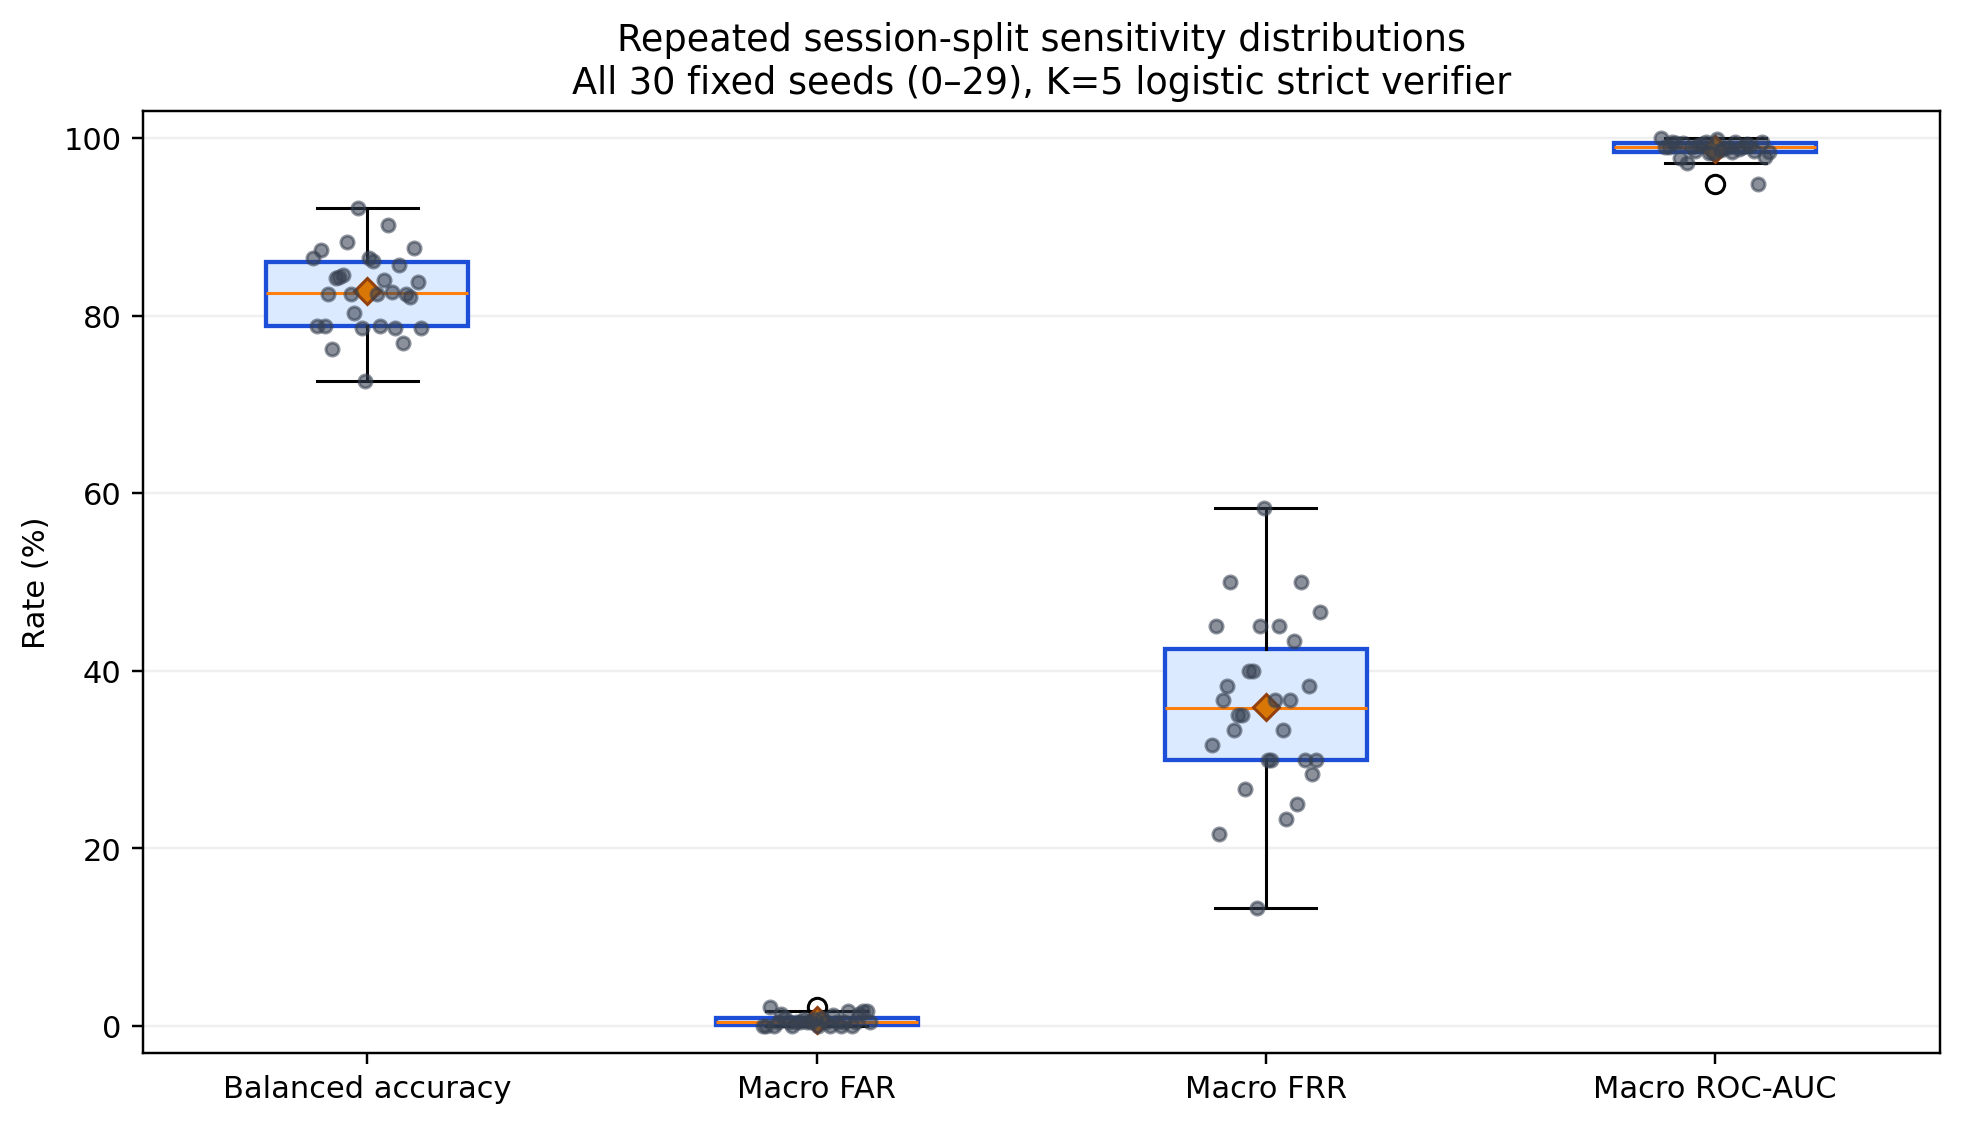
\includegraphics[width=\columnwidth]{sensitivity_distributions.png}
\caption{Metric distributions for all 30 fixed session-separated splits.
Individual points are shown to avoid concealing unfavorable outcomes.}
\label{fig:sensitivity_distributions}
\end{figure}

\begin{figure}[t]
\centering
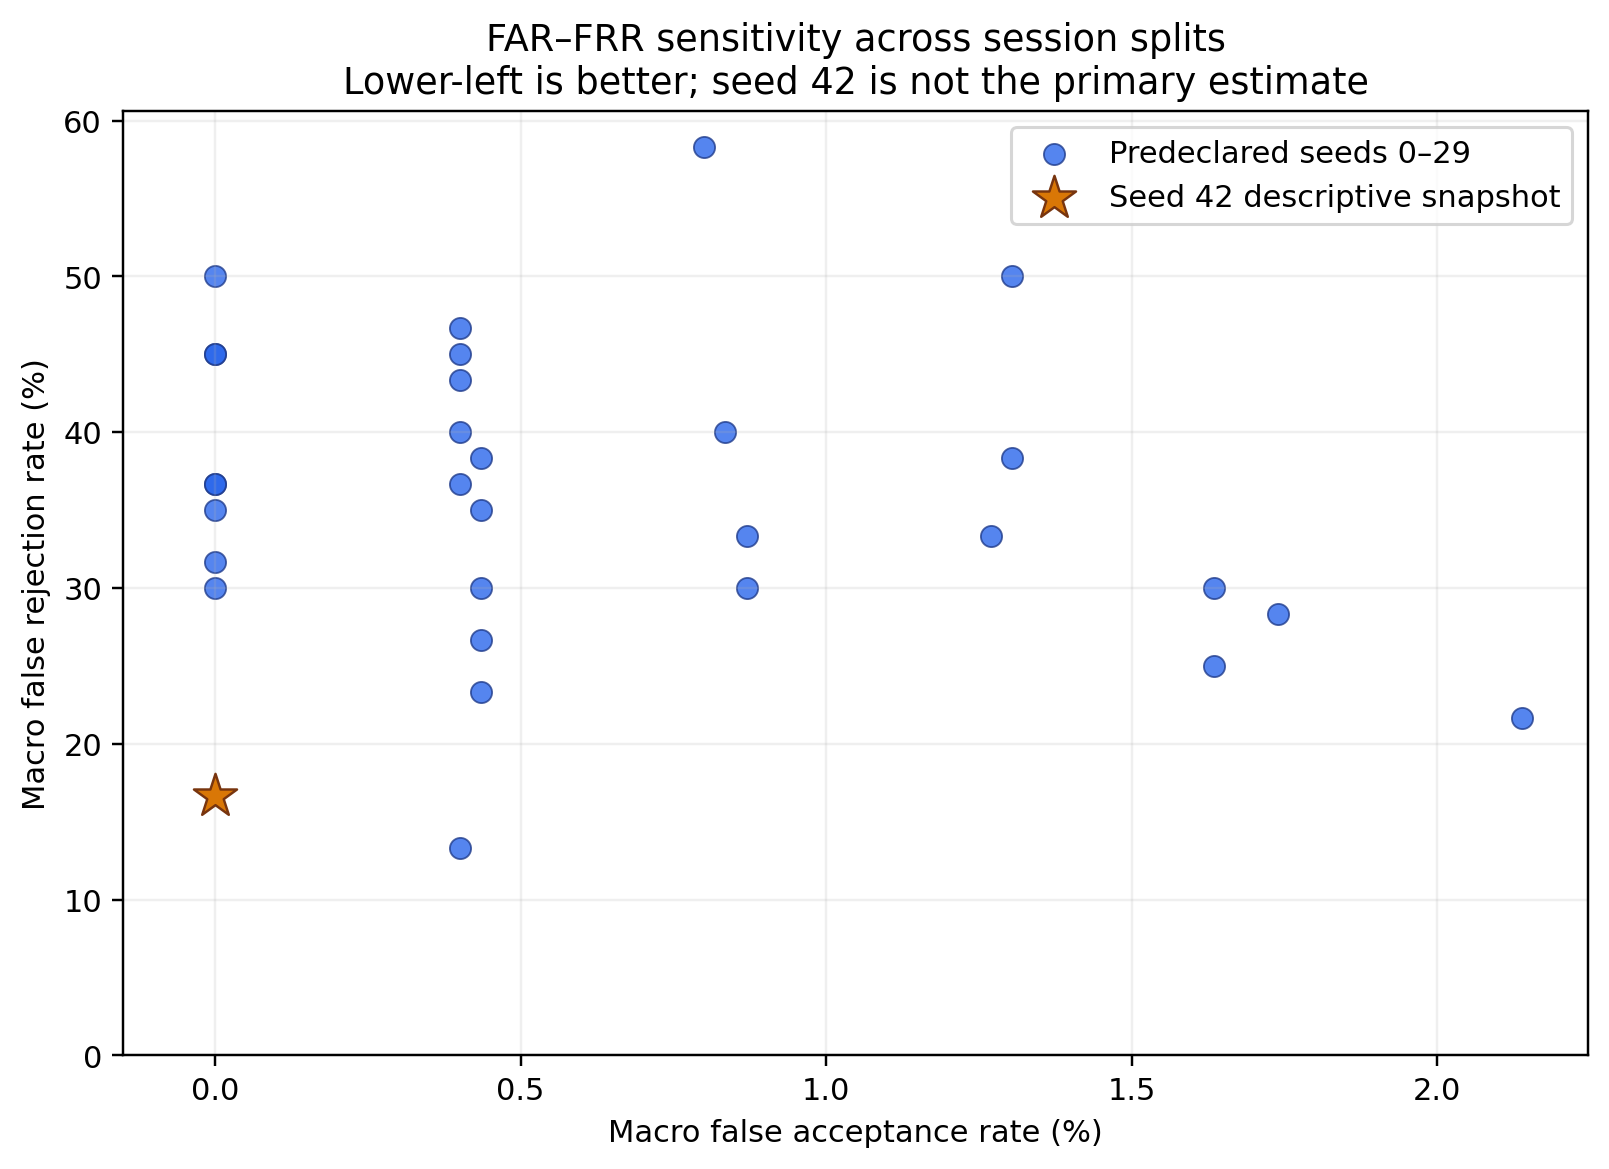
\includegraphics[width=\columnwidth]{sensitivity_far_frr.png}
\caption{Macro FAR and FRR across the fixed split grid. The seed-42 point is
shown for traceability, not selected as the primary estimate.}
\label{fig:sensitivity_far_frr}
\end{figure}

Each seed-42 test attempt was evaluated against its genuine verifier and the
other nine user verifiers, producing 26 genuine and 234 impostor decisions.
Consequently, 90.00\% of decisions were impostor comparisons, and a reject-all
rule would obtain 90.00\% ordinary accuracy. Balanced accuracy, FAR, and FRR
are therefore more informative than ordinary accuracy.

\subsection{Neural Architecture Comparison}

Table~\ref{tab:overall_results} reports the fixed seed-42 neural comparison at
the validation-EER operating point. The GRU-only model achieved lower FAR,
FRR, and EER than the CNN--GRU. The proposed hybrid therefore did not
outperform its component recurrent baseline, and H1 was rejected.

\begin{table*}[t]
\centering
\caption{Seed-42 Neural Verification Performance at $K=5$ (\%)}
\label{tab:overall_results}
\begin{tabular}{lcccccccc}
\toprule
Model & Accuracy & Precision & Recall & F1 & AUC & FAR & FRR & EER \\
\midrule
CNN--GRU & 89.23 & 69.33 & 70.00 & 60.46 & 96.13 & 8.31 & 30.00 & 7.56 \\
CNN-only & 91.15 & 66.77 & 73.33 & 65.24 & 94.45 & 7.34 & 26.67 & 6.79 \\
GRU-only & 93.08 & 67.11 & 80.00 & 68.64 & 96.48 & 5.37 & 20.00 & 4.01 \\
\bottomrule
\end{tabular}
\end{table*}

\begin{figure}[t]
\centering
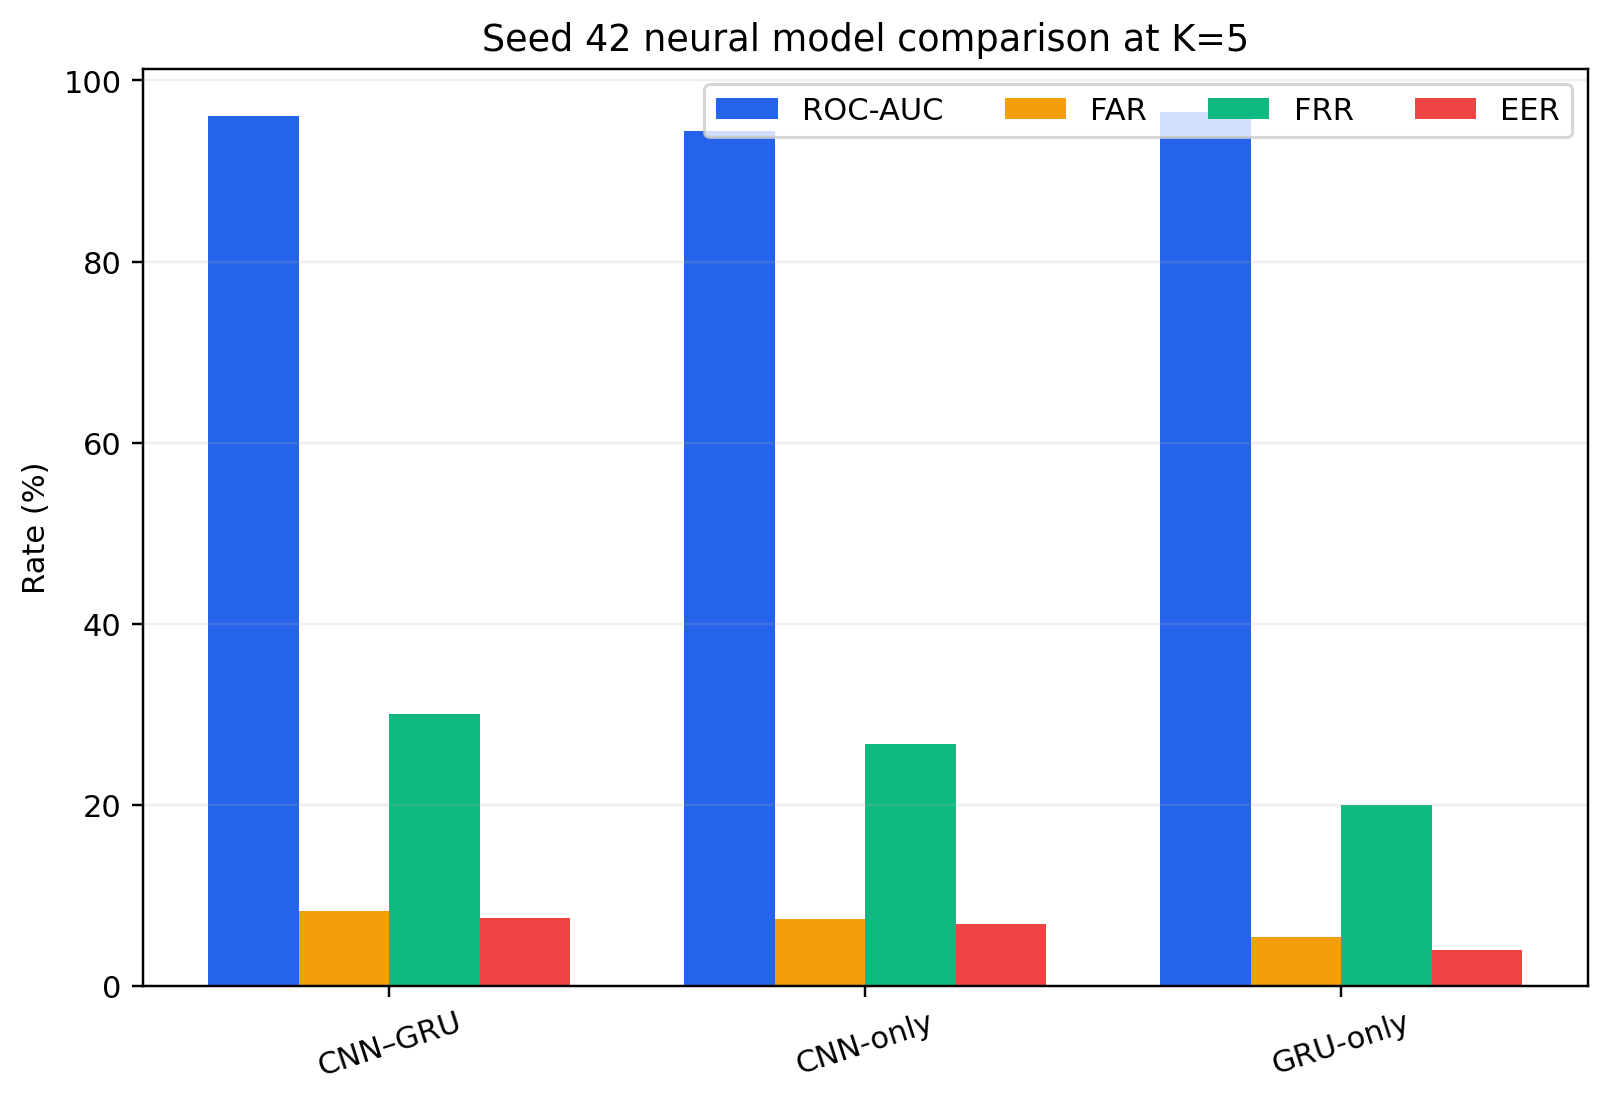
\includegraphics[width=\columnwidth]{neural_model_comparison.png}
\caption{Fixed seed-42 comparison of CNN--GRU, CNN-only, and GRU-only
verifiers.}
\label{fig:neural_comparison}
\end{figure}

\subsection{Classical Baselines}

The classical models were competitive with and sometimes stronger than the
neural architectures. Logistic regression produced the strongest ordinary
accuracy/FAR snapshot, while random forest and gradient boosting achieved low
EER at their balanced thresholds. These rows are descriptive comparisons:
multiple seed-42 test configurations had been inspected during report
development, so none is presented as an untouched selected winner.

\begin{table*}[t]
\centering
\caption{Seed-42 Classical Verification Performance at $K=5$ (\%)}
\label{tab:classical_results}
\begin{tabular}{lcccccccc}
\toprule
Model & Accuracy & Precision & Recall & F1 & AUC & FAR & FRR & EER \\
\midrule
Logistic regression & 96.92 & 95.00 & 83.33 & 86.67 & 99.13 & 1.30 & 16.67 & 1.30 \\
Support-vector machine & 93.46 & 81.50 & 68.33 & 65.81 & 97.90 & 3.37 & 31.67 & 2.14 \\
Random forest & 91.15 & 85.19 & 70.00 & 66.67 & 99.57 & 5.74 & 30.00 & 0.65 \\
$k$-nearest neighbors & 86.54 & 42.82 & 60.00 & 47.40 & 86.05 & 11.18 & 40.00 & 15.64 \\
Gradient boosting & 86.15 & 81.63 & 81.67 & 72.43 & 99.66 & 12.61 & 18.33 & 0.42 \\
\bottomrule
\end{tabular}
\end{table*}

\begin{figure}[t]
\centering
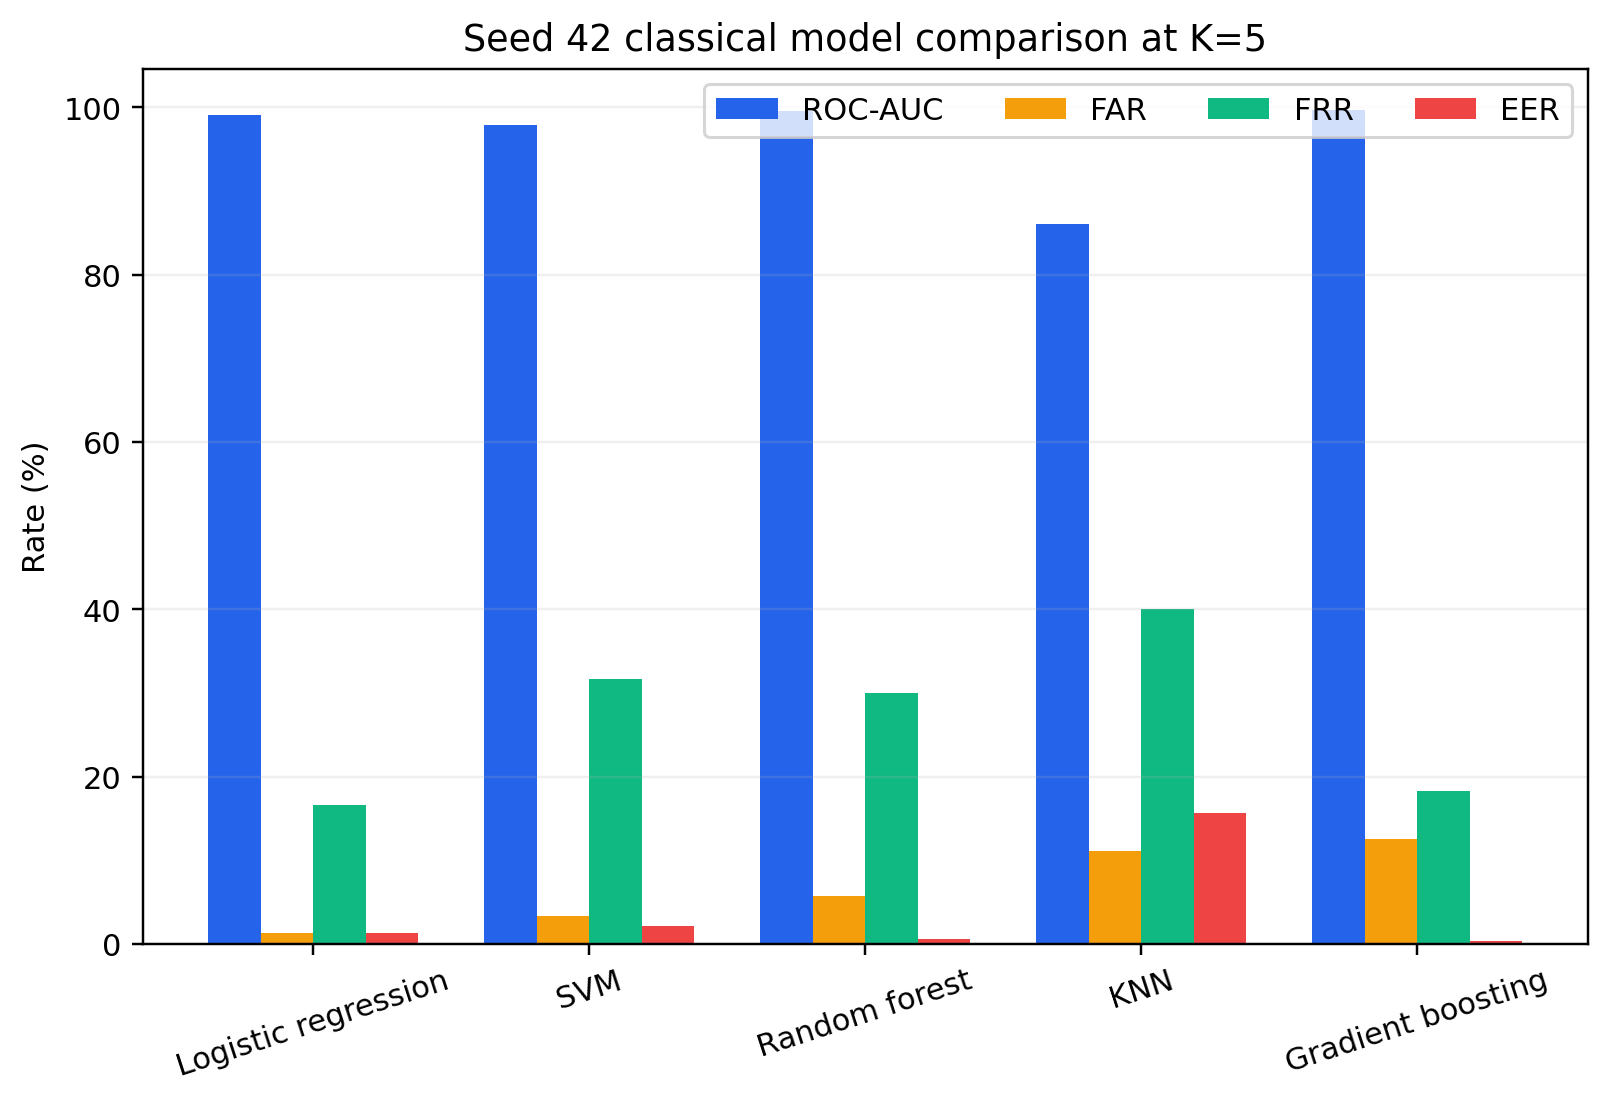
\includegraphics[width=\columnwidth]{classical_model_comparison.png}
\caption{Fixed seed-42 comparison of the five classical baselines.}
\label{fig:classical_comparison}
\end{figure}

\subsection{Effect of the Number of Cursor Movements}

Table~\ref{tab:k_results} reports the repeated strict-logistic tradeoff. Mean
FAR, FRR, and EER improved as more movements were aggregated, but mean duration
increased from 0.98 s at $K=1$ to 4.43 s at $K=5$. The fixed seed-42 CNN--GRU
result was less monotonic: $K=1$, 3, and 5 produced EERs of 13.09\%, 2.91\%,
and 7.56\%, respectively. H2 is therefore partially supported rather than
universally supported.

\begin{table*}[t]
\centering
\caption{Repeated-Split Interaction-Count Tradeoff}
\label{tab:k_results}
\begin{tabular}{ccccccc}
\toprule
$K$ & Mean FAR & Mean FRR & Mean EER & Balanced Accuracy &
Duration (s) & Zero-FP Splits \\
\midrule
1 & 1.71\% & 62.83\% & 10.86\% & 67.22\% & 0.98 & 1/30 \\
3 & 0.93\% & 43.17\% & 5.86\% & 78.95\% & 2.74 & 3/30 \\
5 & 0.63\% & 35.89\% & 1.49\% & 82.82\% & 4.43 & 8/30 \\
\bottomrule
\end{tabular}
\end{table*}

\begin{figure}[t]
\centering
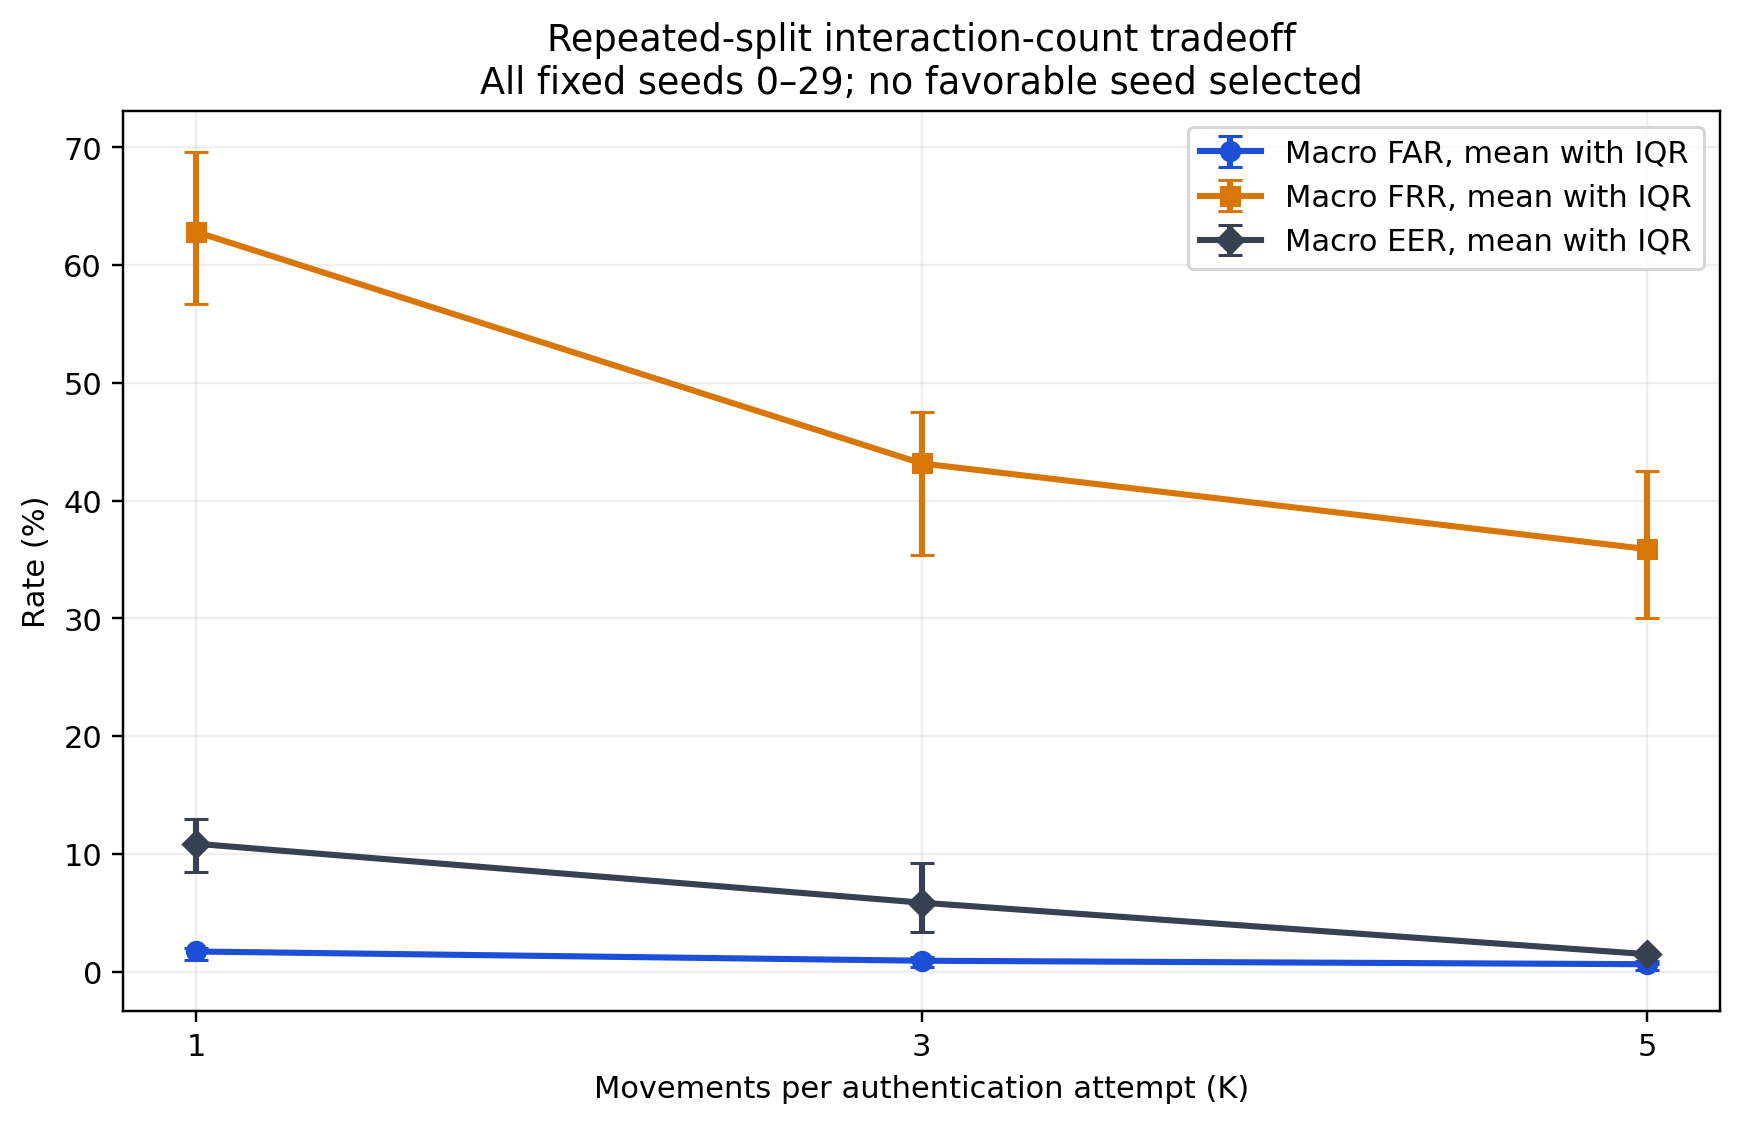
\includegraphics[width=\columnwidth]{repeated_split_k_tradeoff.png}
\caption{Repeated-split interaction-count, error-rate, and duration tradeoff.}
\label{fig:k_tradeoff}
\end{figure}

\subsection{Feature Ablation Results}

The complete target-relative representation improved CNN--GRU AUC and FAR
relative to raw channels, but raw channels achieved a slightly lower EER.
Consequently, H3 produced mixed evidence rather than a uniform improvement.

\begin{table}[t]
\centering
\caption{Seed-42 CNN--GRU Feature Ablation (\%)}
\label{tab:feature_ablation}
\begin{tabular}{lcccc}
\toprule
Features & AUC & FAR & FRR & EER \\
\midrule
Raw & 95.77 & 13.11 & 25.00 & 7.00 \\
Raw + kinematic & 95.72 & 12.07 & 33.33 & 7.64 \\
Full representation & 96.13 & 8.31 & 30.00 & 7.56 \\
\bottomrule
\end{tabular}
\end{table}

\begin{figure}[t]
\centering
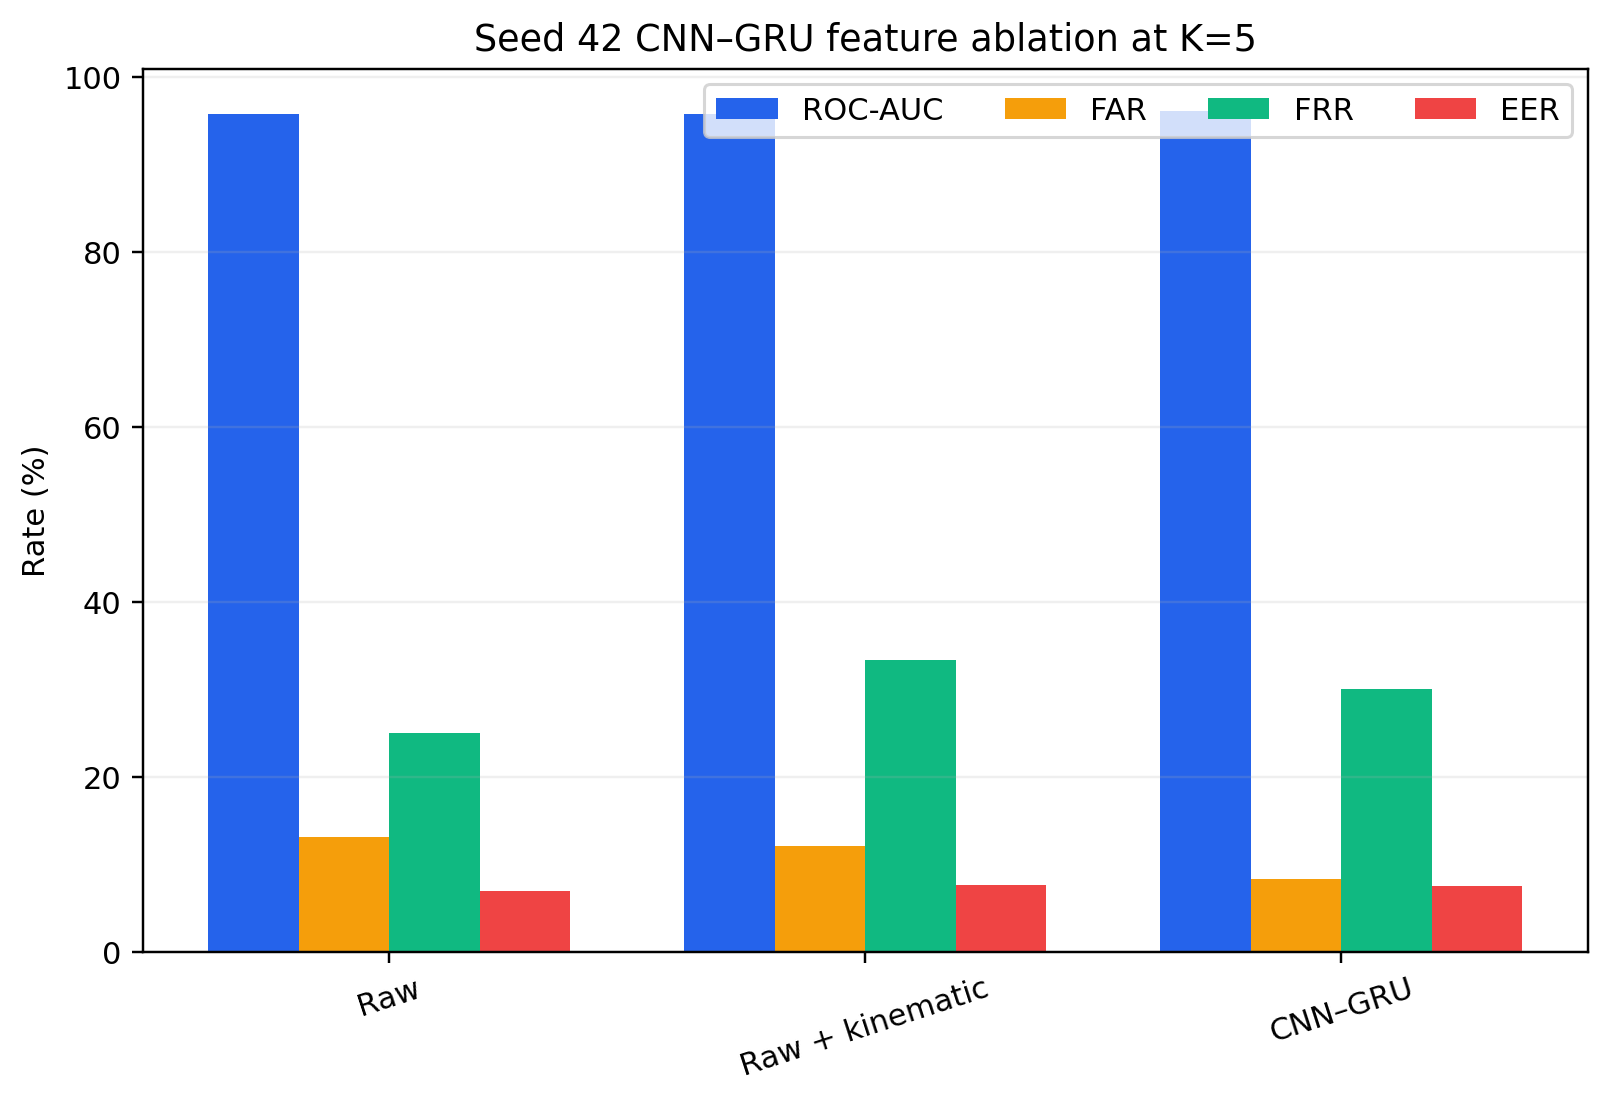
\includegraphics[width=\columnwidth]{feature_ablation.png}
\caption{Fixed seed-42 CNN--GRU feature-ablation results.}
\label{fig:feature_ablation}
\end{figure}

Across the repeated logistic fits, the largest absolute standardized
coefficients were associated with mean and maximum inter-event time, pause
duration, button-state variation, jerk, and click timing. This analysis
describes model influence rather than causal feature importance. The prominence
of timing features also creates a plausible acquisition confound because
browser and device labels were unavailable.

\begin{figure}[t]
\centering
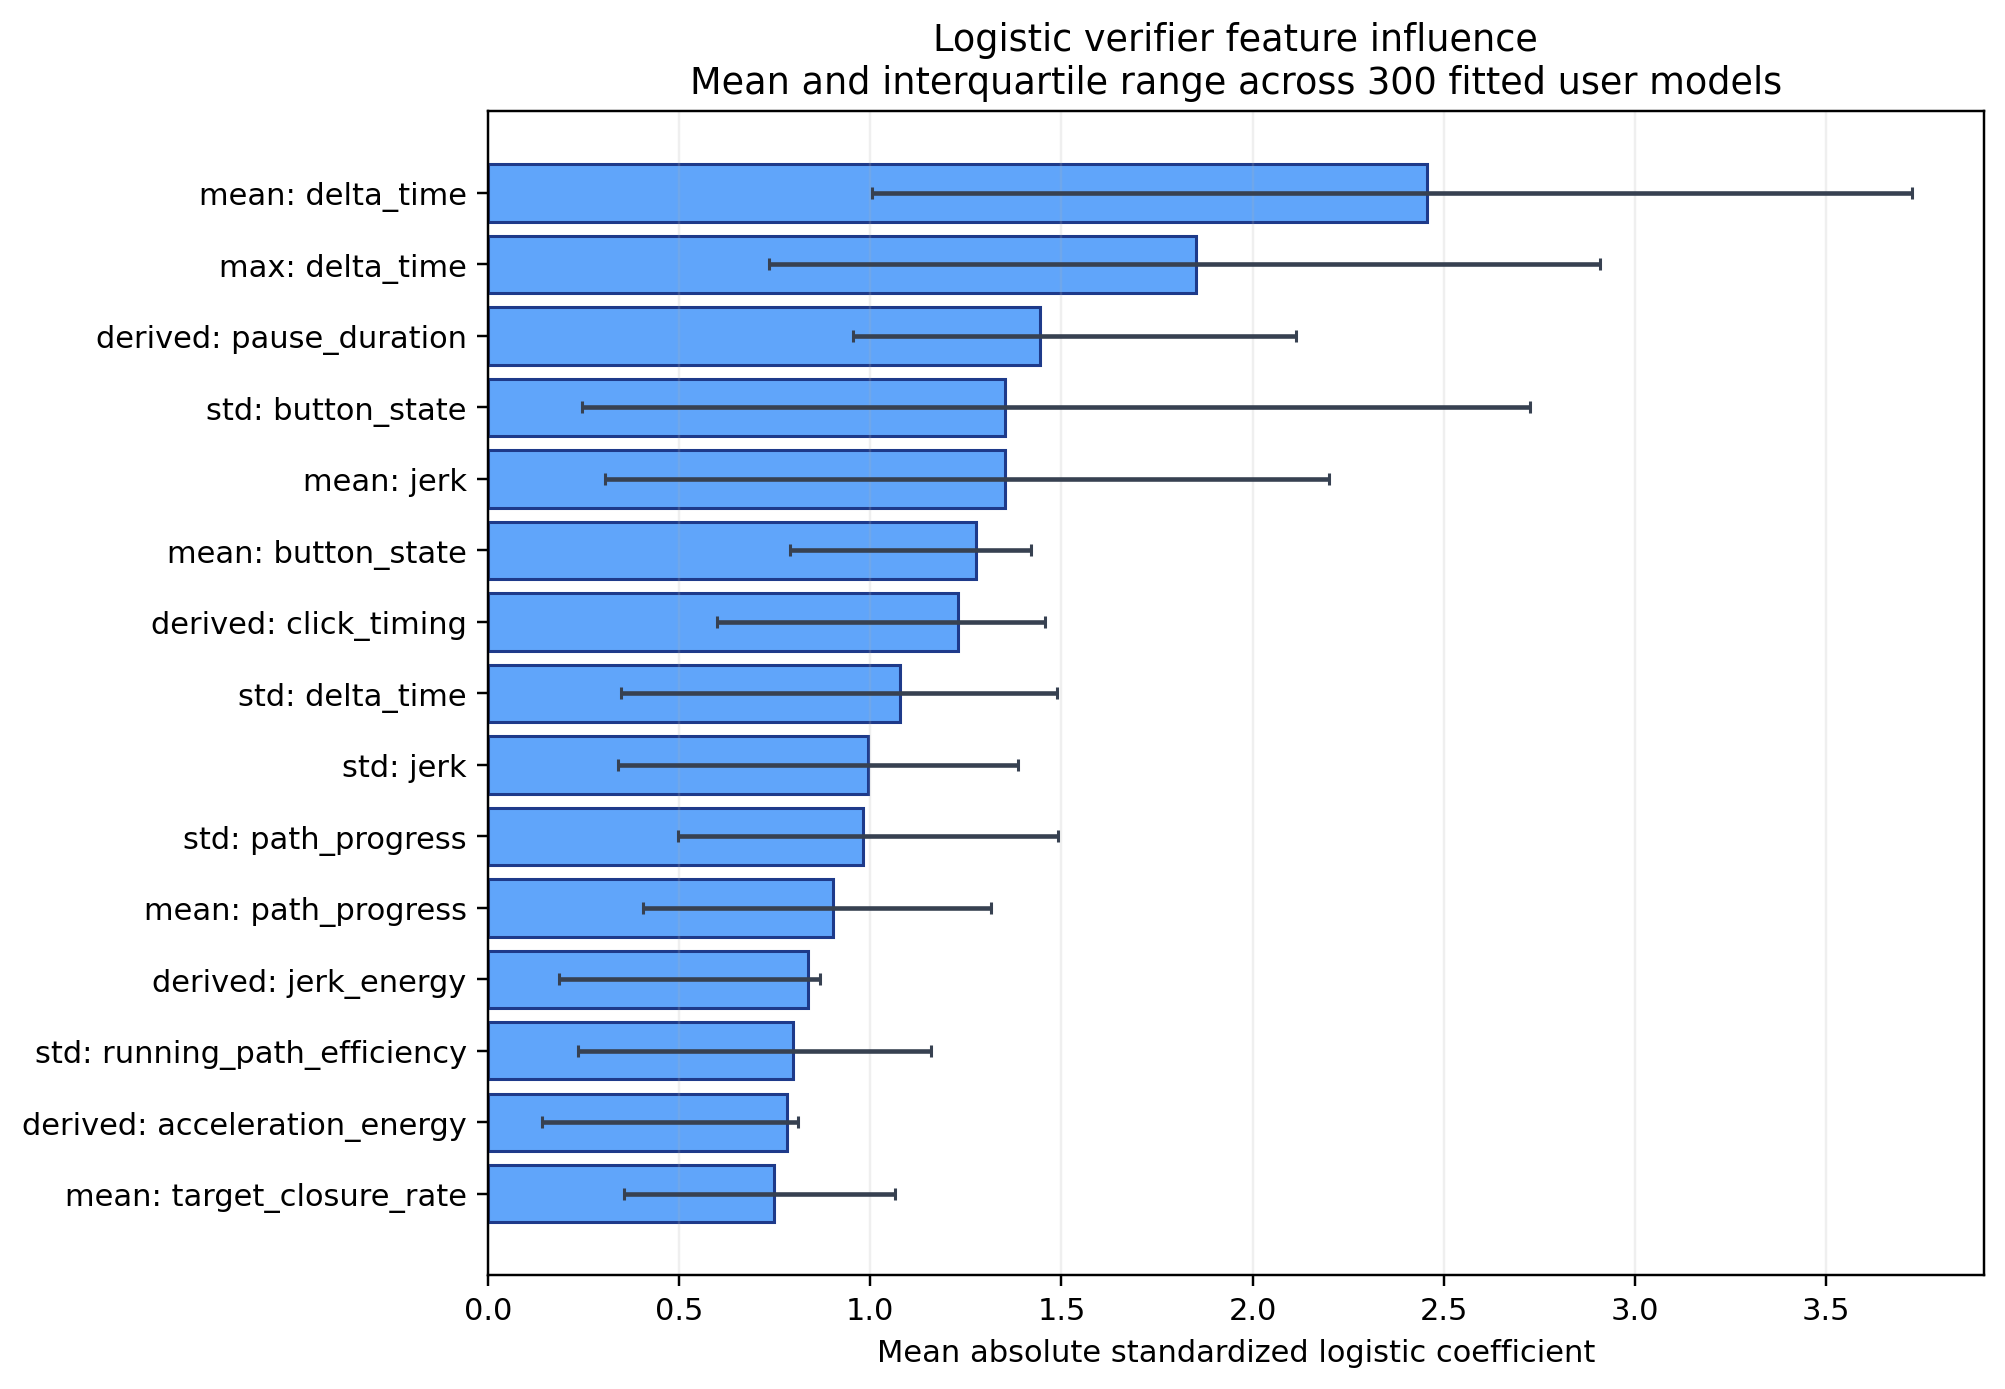
\includegraphics[width=\columnwidth]{feature_influence_logistic.png}
\caption{Mean absolute standardized logistic coefficients across repeated
splits. Error bars show split variation.}
\label{fig:feature_influence}
\end{figure}

\subsection{Session-Separated Evaluation}

The fixed movement-level comparison did not show the expected inflation from
random sample-level splitting. The session-separated evaluation yielded an
AUC of 88.90\%, FAR of 16.33\%, FRR of 19.67\%, and EER of 16.56\%. The random
sample-level evaluation yielded an AUC of 85.96\%, FAR of 20.71\%, FRR of
19.00\%, and EER of 17.19\%. H4 was therefore rejected on this dataset.
This outcome does not make random splitting methodologically preferable;
session separation remains the stronger protection against related-sample
leakage.

\begin{table}[t]
\centering
\caption{Fixed Movement-Level Split Comparison (\%)}
\label{tab:split_comparison}
\begin{tabular}{lcccc}
\toprule
Split & AUC & FAR & FRR & EER \\
\midrule
Session-separated & 88.90 & 16.33 & 19.67 & 16.56 \\
Random sample-level & 85.96 & 20.71 & 19.00 & 17.19 \\
\bottomrule
\end{tabular}
\end{table}

\subsection{Thresholds and Confusion Matrices}

Stricter thresholds reduced false acceptance at the cost of false rejection.
The seed-42 strict logistic snapshot produced 234 true rejects, no false
accepts, five false rejects, and 21 true accepts. Its ordinary accuracy of
98.08\% was aided by the 9:1 impostor/genuine decision imbalance; pooled
balanced accuracy was 90.38\%.

\begin{table*}[t]
\centering
\caption{Seed-42 $K=5$ Operating-Point Comparison (\%)}
\label{tab:operating_points}
\begin{tabular}{lccccrrrr}
\toprule
Configuration & Accuracy & Balanced Accuracy & Macro FAR & Macro FRR &
TN & FP & FN & TP \\
\midrule
CNN--GRU, validation EER & 89.23 & 80.34 & 8.31 & 30.00 & 214 & 20 & 8 & 18 \\
CNN--GRU, strict & 93.85 & 76.07 & 1.69 & 51.67 & 230 & 4 & 12 & 14 \\
Logistic, strict & 98.08 & 90.38 & 0.00 & 16.67 & 234 & 0 & 5 & 21 \\
\bottomrule
\end{tabular}
\end{table*}

\begin{figure}[t]
\centering
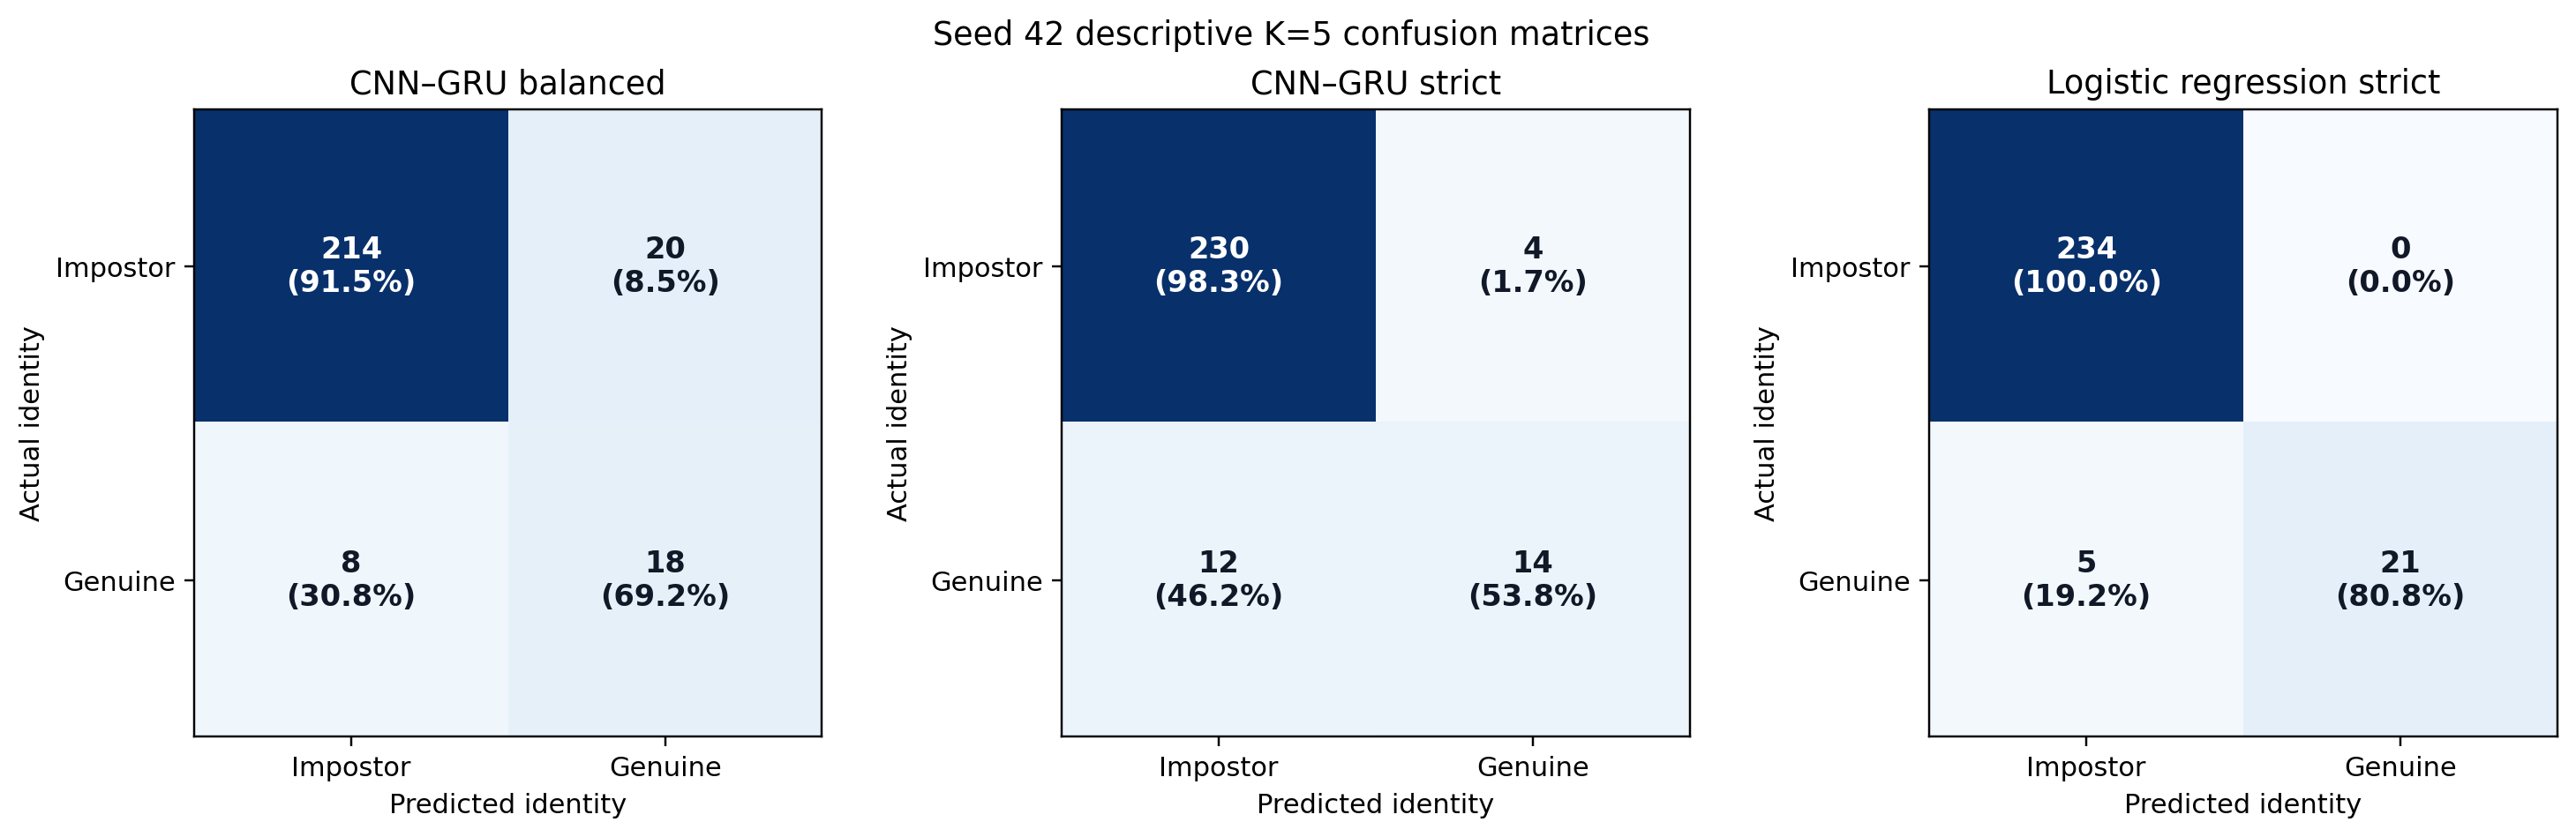
\includegraphics[width=\columnwidth]{confusion_matrix_k5.png}
\caption{Seed-42 confusion matrices for balanced and strict operating points.}
\label{fig:confusion_matrices}
\end{figure}

Zero observed false accepts among 234 impostor decisions is not a population
guarantee. The corresponding one-sided exact 95\% FAR upper bound is 1.2721\%.
Likewise, ROC--AUC measures ranking across thresholds and cannot establish a
deployment-grade rare-event FAR from this sample size.

\subsection{Answers to the Research Questions}

\begin{table*}[t]
\centering
\caption{Research-Question and Hypothesis Outcomes}
\label{tab:rq_outcomes}
\begin{tabular}{lll}
\toprule
\textbf{Item} & \textbf{Outcome} & \textbf{Evidence} \\
\midrule
RQ1/H1 & Rejected & GRU-only EER 4.01\%; CNN--GRU EER 7.56\% \\
RQ2/H2 & Partial & More movements help repeated means; neural result is nonmonotonic \\
RQ3/H3 & Mixed & Full features improve AUC/FAR but not EER \\
RQ4 & Confirmed tradeoff & Strict thresholds lower FAR while increasing FRR \\
RQ5 & Not stable & $K=5$ FAR 0.00--2.14\%; FRR 13.33--58.33\% \\
RQ6 & Not established & Hardware, device, DPI, browser labels unavailable \\
H4 & Rejected here & Random sample-level metrics were not better \\
\bottomrule
\end{tabular}
\end{table*}

\section{Discussion}

\subsection{Interpretation of Results}

The most compelling evidence provided by this study is derived from the comprehensive distribution across 30 distinct data splits rather than the isolated and relatively favorable results obtained from the seed-42 strict logistic configuration. Although a mean macro ROC--AUC of 98.78\% indicates a robust capacity for identity ranking, the mean macro FRR of 35.89\%---with substantial variation from 13.33\% to 58.33\%---shows that the strict operating point remains unstable and would likely cause significant friction for legitimate users. Therefore, these results substantiate the potential of mouse dynamics as a supplemental authentication signal but indicate that the technology is not currently suitable for deployment as a primary or standalone security factor.

Contrary to initial hypotheses, the anticipated performance superiority of the CNN--GRU architecture was not realized during evaluation. In the fixed neural comparison, the GRU-only model achieved superior metrics with lower FAR, FRR, and EER values, while several classical baseline configurations demonstrated competitive performance. Furthermore, experiments involving interaction-count variations and feature-ablation studies produced heterogeneous outcomes rather than consistently favorable trends. These negative results are deliberately retained within the analysis, as the selective reporting of only the optimal model, feature subset, or data split would constitute an unjustifiable overstatement of the empirical evidence.

\subsection{Comparison with Prior Mouse-Dynamics Results}

Table~\ref{tab:prior_work_comparison} presents the findings from NeuroCursor alongside a selection of established results in the field of mouse-dynamics authentication. It is important to note that these figures are intended to offer numerical context rather than serve as a definitive ranking. The reason is that comparing them directly is difficult due to the wide variety of methodologies used across different studies. Specifically, researchers often employ different datasets and interaction tasks, while the lengths of decision units and the strategies for constructing negative samples also vary. Furthermore, differences in class balance, data split procedures, and the specific methods used for threshold calibration mean that these results exist within their own distinct experimental frameworks.

\begin{table*}[t]
\centering
\small
\caption{Numerical Context from Prior Mouse-Dynamics Studies. These Results
Do Not Constitute a Head-to-Head Benchmark.}
\label{tab:prior_work_comparison}
\begin{tabular}{@{}>{\raggedright\arraybackslash}p{2.4cm}
                    >{\raggedright\arraybackslash}p{4.8cm}
                    >{\raggedright\arraybackslash}p{2.5cm}
                    cccc@{}}
\toprule
\textbf{Study} &
\textbf{Dataset and Evaluation} &
\textbf{Decision Unit} &
\textbf{AUC (\%)} &
\textbf{EER (\%)} &
\textbf{FAR (\%)} &
\textbf{FRR (\%)} \\
\midrule
\textbf{NeuroCursor} &
10 identities; randomized challenge; 30 session-separated logistic fits &
5 directed movements &
98.78 &
1.49 &
0.63$^{*}$ &
35.89$^{*}$ \\

Antal and Fej\'er \cite{antalFejer2020} &
Balabit; 10 users; 1D-CNN authentication &
All available blocks; 128 mouse events &
98.00 &
-- &
-- &
-- \\

Antal and Egyed-Zsigmond \cite{antalEgyed2019} &
Balabit benchmark test data; scenario B; set-of-actions evaluation &
20 mouse actions &
89.94 &
18.80 &
-- &
-- \\

Wang \textit{et al.} \cite{wang2025Mouse} &
Balabit; LT-AMouse blind-attack evaluation &
MAU length 90--130 &
97.73 &
6.14 &
-- &
-- \\
\bottomrule
\end{tabular}

\vspace{1mm}
\begin{minipage}{0.97\textwidth}
\footnotesize

$^{*}$ The NeuroCursor FAR and FRR are calculated at the strict operating point calibrated on the validation set. The EER is calculated separately from the score distributions and is therefore not measured simultaneously with the reported strict FAR and FRR. A dash indicates that the cited study did not report the corresponding metric for the listed configuration.
\end{minipage}
\end{table*}

In terms of numerical performance, the mean ROC--AUC of 98.78\% achieved by NeuroCursor is comparable to the 98.00\% AUC reported by Antal and Fej\'er and the 97.73\% AUC cited for LT-AMouse. Although the mean EER for NeuroCursor (1.49\%) appears lower than the EER values associated with these external configurations, such differences should not be viewed as definitive evidence of statistical superiority. NeuroCursor uses a restricted, randomized challenge and a specific ten-identity cohort, whereas the benchmark studies rely on fundamentally different datasets and evaluation frameworks. Additionally, the strict operating point for NeuroCursor resulted in a mean FRR of 35.89\%, highlighting a notable usability tradeoff despite the strong classification metrics. Ultimately, a rigorous claim of superiority would require a head-to-head evaluation in which all systems are tested using identical data splits, decision units, and calibration procedures.

The reported metrics for LT-AMouse are derived from Table III of \cite{wang2025Mouse}, which provides Balabit F1, AUC, and EER values of 94.65\%, 97.73\%, and 6.14\%, respectively. Although the abstract of that study identifies 94.65\% as the Balabit AUC, the more granular data from the comparison table are used here to identify the source of these values precisely.

\subsection{Security and Usability Implications}

NeuroCursor is most appropriately categorized as a supplemental authentication signal within a multilayered security framework. In practice, a low behavioral score could trigger step-up authentication rather than an immediate denial of access. Increasing the number of movements $K$ improved the repeated strict-verifier averages, but the mean challenge duration increased from 0.98 s at $K=1$ to 4.43 s at $K=5$. Furthermore, a stricter threshold reduced FAR while increasing FRR. Consequently, a deployment threshold must account for the threat model, accessibility requirements, account-recovery costs, and the relative operational consequences of false acceptance and false rejection.

\subsection{Threat Model and Operational Scope}

The present evaluation focuses on verifying claimed identities against typical human impostors. In this context, an impostor sample is simply a real cursor trajectory from one participant that is tested against a different user's verifier. This setup is meant to see if the natural differences in how people move their cursors are enough to tell them apart. It is important to note, however, that this doesn't prove the system can stop a determined attacker who might record and replay a user's movements, inject fake events, mimic someone's style, or mess with the browser and device settings.

This distinction is key when interpreting the reported False Acceptance Rate (FAR). The mean macro FAR we found in the repeated strict-logistic tests only describes the errors within this specific group and their particular testing conditions. Even in cases where we saw zero false accepts in a split, that doesn't mean the actual population FAR is zero. For instance, the seed-42 result had 234 impostor decisions with zero errors, which translates to a one-sided exact 95\% FAR upper bound of 1.2721\%. To prove the system works at much rarer error rates, we would need a significantly larger pool of independent impostor trials collected under a pre-set testing protocol \cite{isoBiometricTesting}.

\begin{table*}[t]
\centering
\caption{Threat-Model Coverage and Residual Validation Requirements}
\label{tab:threat_model_coverage}
\begin{tabular}{@{}p{3.1cm}p{5.6cm}p{6.3cm}@{}}
\toprule
\textbf{Threat or Variation} &
\textbf{Coverage in the Present Study} &
\textbf{Required Future Validation} \\
\midrule
Ordinary human impostor &
Attempts from other enrolled identities are evaluated against each claimed
identity's verifier. &
Evaluate a larger external cohort with identities that were not involved in
model development or report preparation. \\

Related-sample leakage &
All movements from one session remain within the same training, validation, or
test subset. &
Conduct longitudinal evaluation with collection periods separated by days,
weeks, or months. \\

Split sensitivity &
The complete strict-logistic pipeline is refitted across the fixed seed grid
from 0 to 29. &
Confirm the observed distribution using a preregistered protocol and an
untouched replication cohort. \\

Replay or event injection &
Not represented in the supplied dataset. &
Test recorded-event replay, synthetic pointer injection, timestamp
manipulation, and browser-level automation. \\

Deliberate behavioral imitation &
Not represented in the supplied dataset. &
Collect informed imitation attempts after adversaries observe examples of an
enrolled user's trajectories. \\

Device and environment variation &
Hardware, input-device, DPI, sensitivity, and browser labels are unavailable. &
Collect controlled cross-device and cross-browser sessions with complete
acquisition metadata. \\

Rare-event false acceptance &
Observed through the available impostor decisions and reported with a finite-
sample upper bound. &
Perform high-volume impostor testing sufficient to estimate the intended
deployment FAR with an appropriate confidence bound. \\
\bottomrule
\end{tabular}
\end{table*}

A practical deployment should therefore situate NeuroCursor within a multi-layered authentication framework. A high verification score may serve as corroborating evidence for a claimed identity, whereas a low or indeterminate score could necessitate the invocation of a secondary authentication factor. Such an architecture ensures that a probabilistic behavioral measurement is not treated as an irrevocable access decision. Furthermore, this design provides a robust mechanism for accommodating legitimate behavioral variances resulting from fatigue, injury, temporary impairment, unfamiliar hardware configurations, or fluctuations in environmental conditions.

Operational evaluation must additionally consider accessibility and differential performance across user populations. A singular, global interaction design may not provide equivalent usability for participants with varying motor abilities, different pointing devices, or disparate levels of task familiarity. While user-specific thresholds partially mitigate differences in score distributions, they do not serve as a substitute for dedicated accessibility research. Consequently, future deployment-oriented studies should report rates of enrollment and verification failure, task completion times, and error distributions across relevant user and device demographics in conjunction with aggregate biometric metrics.

\subsection{Proposed External Validation Protocol}

A confirmatory evaluation should be finalized prior to any further model selection or threshold adjustments. Such a study must recruit an external cohort consisting of participants, sessions, and behavioral samples that were entirely absent during the initial development of NeuroCursor. Before data acquisition commences, investigators should preregister the intended sample size, criteria for inclusion and exclusion, session architecture, movement-count configurations, the primary operating point, and the comprehensive statistical analysis plan. Furthermore, cohort size should be determined by an a priori power analysis, and all biometric testing and reporting should adhere strictly to the established principles of ISO/IEC 19795-1 \cite{cohenPower,isoBiometricTesting}.

Data collection should systematically document the pointing device, operating system, browser, display resolution, cursor sensitivity, and—where available—DPI, along with participant handedness and relevant accessibility conditions. To ensure the evaluation assesses longitudinal stability rather than short-term repetition, each participant should complete multiple sessions distributed over several days or weeks. Furthermore, the protocol should incorporate controlled cross-device and cross-browser sessions. All samples derived from a single participant session must be maintained within the same data split, and the final test cohort must remain inaccessible until the feature set, model configuration, aggregation rules, and calibration procedures have been finalized and locked.

The external evaluation should maintain a strict distinction between ordinary human impostors and deliberate adversarial attacks. Dedicated test sets should examine replayed trajectories, synthetic event injection, and informed imitation conducted after an attacker observes representative movements. Given that claims regarding rare-event false-acceptance rates require substantially more independent impostor decisions than the current dataset provides, the FAR should be reported alongside exact binomial confidence bounds. This practice must include cases with zero observed false accepts to ensure the metric is not interpreted solely from the point estimate \cite{clopperPearson}.

Performance reporting should encompass ROC--AUC, EER, FAR, FRR, accuracy, balanced accuracy, and confusion counts at the prespecified operating point. Results must be presented both in aggregate and disaggregated by participant, session, device category, and movement count. Furthermore, confidence intervals and bootstrap estimates should accompany the principal metrics where appropriate \cite{efronBootstrap}. Adherence to this protocol would provide a substantially stronger basis for assessing generalization, usability, and security, thereby positioning the present study as an exploratory development evaluation rather than as definitive confirmatory evidence.

\subsection{Operational Deployment Decision Framework}

A deployment-oriented iteration of NeuroCursor necessitates an explicit decision policy to complement its classification capabilities. The verification system should not automatically translate every low-confidence score into an immediate denial of access. Instead, the application architecture should define at least three distinct outcomes: provisional acceptance for scores exceeding a high-confidence threshold; step-up authentication for scores residing within a predefined uncertainty region; and rejection or temporary restriction only when both behavioral evidence and an independent security signal justify such a response. This tripartite structure preserves the supplemental role of behavioral biometrics and mitigates the risk that ordinary variation in a legitimate user's movement triggers an irreversible access decision \cite{nistBiometrics,deutschmannContinuousAuthentication}.

Threshold selection should be informed by the operational costs associated with false acceptance and false rejection, rather than a single global performance statistic. For instance, financial or administrative systems may assign a higher cost to unauthorized access, whereas educational or low-risk applications may prioritize continuity of service. The chosen policy must therefore document the validation population, the score-aggregation rule, the threshold-calibration objective, the permitted number of retries, and the specific authentication factor invoked following an indeterminate result. These parameters must be finalized using only training and validation data; the held-out test cohort should be reserved for a single final assessment. Reporting multiple post hoc test thresholds should be avoided, as it obscures the intended operating point and overstates statistical certainty.

Enrollment and template maintenance procedures require a strictly defined lifecycle to ensure system integrity. The initial enrollment phase must incorporate multiple sessions and a robust quality-assurance check designed to identify incomplete trajectories, extreme timing artifacts, or insufficient behavioral coverage. If the resulting template fails to satisfy predetermined quality criteria, the system should document a failure-to-enroll outcome rather than programmatically constructing an unreliable verifier. Subsequent template updates should be restricted to instances where the user has completed a session authenticated via an independent factor. Furthermore, each update should be versioned so that abrupt score degradation, suspected compromise, or device migration can trigger a formal review or rollback. Finally, implementing a fixed expiration or reevaluation interval would prevent an outdated template from being treated as a permanently representative model of user behavior.

Operational monitoring should distinguish model error from acquisition failure and user-interface failure. Recommended measures include failure-to-enroll rate, failure-to-acquire rate, retry frequency, challenge-completion time, step-up frequency, recovery success, and the distribution of scores across supported devices. These outcomes should be examined by participant and device category, subject to appropriate privacy protections, because an acceptable aggregate average can conceal severe difficulty for a subset of users. Monitoring should also detect sustained score drift without automatically labeling that drift as malicious; injury, fatigue, unfamiliar hardware, and accessibility-related changes may produce legitimate departures from an earlier template.

The deployment architecture should minimize retained behavioral data, encrypt stored templates, restrict access to raw trajectories, and maintain auditable records of model and threshold versions. Users should receive clear notice that cursor behavior contributes to authentication and should retain access to a conventional recovery mechanism. Evaluation of the complete policy—not merely the classifier—would align the reported biometric metrics with the practical reliability, security, accessibility, and accountability requirements of a real authentication system \cite{isoBiometricTesting}.

The implementation of a staged deployment strategy should prioritize a meticulously monitored pilot phase, eschewing immediate, organization-wide integration in favor of a controlled rollout. To ensure operational integrity, the system must incorporate predefined cessation criteria that mandate the suspension of the verification framework whenever empirical metrics—such as false-rejection rates, recovery failures, or sustained score drift—exceed the specific tolerance thresholds established during validation.

Finally, the administrative responsibility for evaluating these alerts must be clearly assigned to qualified personnel prior to the initiation of the deployment. Maintaining robust human oversight is of paramount importance when behavioral evidence influences account accessibility; this is because automated monitoring protocols currently lack the nuanced discernment required to reliably differentiate between a malicious security compromise and legitimate, non-adversarial shifts in a user's physical or environmental circumstances.

\subsection{Limitations}

This investigation is subject to several critical limitations. The evaluable cohort is restricted to 10 anonymized identities and 266 sessions; notably, one identity contributed only three eligible sessions, causing certain validation and test rates to remain highly discrete. Although 30 repeated splits were conducted, they reuse the same restricted cohort and measure split sensitivity rather than population generalization. Furthermore, participant provenance and the authenticity of the data-collection process were not independently verified. Because metadata regarding hardware, input-device type (e.g., mouse versus trackpad), DPI settings, sensitivity, browser environment, handedness, fatigue, injury, and environmental conditions were unavailable, the study could not evaluate cross-device robustness or acquisition-related variability. The dataset also lacked recordings of replay or deliberate-imitation attacks, and the impostor sample size is insufficient to establish deployment-grade false acceptance rates for rare events. Finally, because multiple seed-42 model configurations and threshold outcomes were inspected during preparation of this report, a completely untouched external cohort is necessary for rigorous confirmatory evaluation.

\subsection{Ethical and Privacy Considerations}

Behavioral biometrics should be treated as a sensitive modality because they may reflect distinctive patterns of user interaction. A practical system should minimize unnecessary data collection, store only the data required for authentication, protect stored templates, and provide clear notice to users.

This research project was conducted under the supervision and direct approval of faculty and staff at The University of Texas at Dallas. The dataset used for this analysis was provided with anonymized identity labels to protect participant privacy. This statement documents academic oversight and does not constitute an assertion of formal Institutional Review Board (IRB) approval, exemption, or waiver.

\section{Conclusion}

This paper presents NeuroCursor, a behavioral biometric verification framework based on randomized mouse-movement challenges. The system records cursor trajectories during users' point-and-click interactions, represents the trajectories as multivariate time series, and evaluates whether user-specific movement patterns can support authentication. We present NeuroCursor not as the first mouse-dynamics authentication system or the first CNN--GRU approach, but as an experimental study of a short randomized protocol, target-relative feature representation, interaction-count tradeoffs, and session-aware evaluation.

Evaluation across the fixed 30-split sensitivity grid revealed that the strict full-feature logistic verifier, when utilizing a five-movement sequence, achieved a mean pooled balanced accuracy of 82.82\%, a mean macro FAR of 0.63\%, a mean macro FRR of 35.89\%, and a mean macro ROC--AUC of 98.78\%. Notwithstanding these aggregate metrics, empirical performance exhibited material variance across individual splits, and the CNN--GRU architecture failed to demonstrate statistical superiority over either the GRU-only baseline or the most robust classical models. These findings substantiate NeuroCursor as a rigorous framework for the ongoing investigation of supplemental behavioral verification, yet they simultaneously indicate that the system is not currently a deployment-ready replacement for established authentication factors. Future research must incorporate a substantially larger and untouched cohort, longitudinal and cross-device acquisition metadata, high-volume rare-event impostor trials, comprehensive accessibility assessments, and rigorous testing against explicit replay and imitation attacks.

\FloatBarrier

\appendix[Implementation Traceability]

Table~\ref{tab:implementation_traceability} maps the principal mathematical
and experimental components of NeuroCursor to their corresponding
implementation functions.

\begin{table*}[t]
\centering
\caption{Paper-to-Implementation Traceability}
\label{tab:implementation_traceability}
\begin{tabular}{lll}
\toprule
\textbf{Paper Component} &
\textbf{Equation or Section} &
\textbf{Implementation Function} \\
\midrule

Feature extraction &
Feature Engineering &
\texttt{engineer\_raw\_features} \\

Sequence interpolation &
Eq.~\ref{eq:sequence_interpolation} &
\texttt{resample\_sequence} \\

Training normalization &
Eq.~\ref{eq:zscore_normalization} &
\texttt{fit\_standardizer}, \texttt{standardize} \\

Session separation &
Experimental Methodology &
\texttt{create\_split}, \texttt{\_group\_split} \\

CNN--GRU model &
CNN--GRU Architecture &
\texttt{build\_model} \\

Binary cross-entropy &
Eq.~\ref{eq:bce_loss} &
Keras binary-cross-entropy objective \\

Class balancing &
Eq.~\ref{eq:class_weight} &
\texttt{class\_weights} \\

Classical feature summaries &
Baselines and Ablation Studies &
\texttt{summarize\_sequences} \\

Attempt aggregation &
Eq.~\ref{eq:aggregate_score} &
\texttt{aggregate\_attempt\_scores} \\

Validation-EER calibration &
Threshold Calibration &
\texttt{calibrate\_eer\_threshold} \\

Strict threshold calibration &
Threshold Calibration &
\texttt{calibrate\_far\_threshold} \\

Biometric metrics &
Eqs.~\ref{eq:accuracy}--\ref{eq:eer} &
\texttt{biometric\_metrics} \\

Repeated-split robustness &
Results &
\texttt{sensitivity} \\

\bottomrule
\end{tabular}
\end{table*}

\section*{AI-Assisted Development Disclosure}

The initial conception of NeuroCursor, the design of its data-acquisition framework, and the selection of the CNN--GRU architecture arose from the authors' independent research. The core implementation and experimental methodology were likewise completed by the authors prior to the introduction of automated assistance. OpenAI Codex, accessed through the ChatGPT desktop interface using the GPT-5.6 Sol model, was subsequently employed in a limited supplementary capacity. Its technical contribution was confined to assisting with the implementation of a small number of additional engineered features and the configuration of the $K=1$, $K=3$, and $K=5$ evaluation workflows \cite{openaiCodexModels}. All such extensions were specified, reviewed, and empirically verified by the authors, who independently interpreted the resulting data and retain sole responsibility for the methodology, findings, conclusions, and submitted manuscript.

\section*{Author Contributions}

\textbf{Shaurya Saxena:} Lead authorship, research direction, and primary
responsibility for the preparation, organization, and revision of the
manuscript, including the literature review, mathematical formulation,
experimental methodology, results, discussion, and final presentation of the
research. Additional contributions included project conceptualization,
particularly the framing of NeuroCursor as a supplemental two-factor or
multi-factor authentication mechanism; development of the research outline,
prepared in advance, that defined the proposed workflow and evaluation
framework;
presentation development; mathematical feature design; experimental
evaluation; formal analysis; validation of reported findings; and
interpretation of results.

\textbf{Hamid Abdu Mossa:} Original project conceptualization and primary
technical responsibility for the design and development of NeuroCursor,
including its model architecture and end-to-end software system. He led the
detailed design, refinement, implementation, and integration of the
machine-learning model, translating the research outline and project
requirements into an operational architecture. His contributions also
included backend and frontend development, machine-learning pipeline
integration, end-to-end system integration, software testing and debugging,
and contributions to experimental analysis and interpretation of results.

\textbf{Shreehan Aalok Pathak:} Frontend design and development, including
the implementation of interactive interface components and integration of
the user interface with the broader NeuroCursor workflow. Additional
contributions included supporting model development and model-to-interface
integration.

\textbf{Chetan Gangireddy:} Early contributions to model-architecture
development, including participation in the initial exploration of model
designs and system requirements. Additional contributions included
background research, the ideation of candidate behavioral features, and
support for data loading and initial data-ingestion workflows.

All authors reviewed the completed work, approved the final manuscript, and
accept responsibility for their respective contributions.

\section*{Acknowledgment}
The authors gratefully acknowledge Dr. Anurag Nagar for his guidance and mentorship throughout this research process. The authors also thank Hamid Rouhani, a Ph.D. student in computer science at The University of Texas at Dallas, for his valuable research guidance and support.

\FloatBarrier

\begin{thebibliography}{99}

\bibitem{nistBiometrics}
National Institute of Standards and Technology,
``Biometrics,''
\emph{Computer Security Resource Center Glossary}.
[Online]. Available: \url{https://csrc.nist.gov/glossary/term/Biometrics}.
Accessed: Jul. 2026.

\bibitem{khanMouseSurvey}
S. Khan, C. Devlen, M. Manno, and D. Hou,
``Mouse dynamics behavioral biometrics: A survey,''
\emph{ACM Computing Surveys},
vol. 56, no. 6, Art. no. 154, 2024,
doi: 10.1145/3640311.

\bibitem{deutschmannContinuousAuthentication}
I. Deutschmann, P. Nordstr{\"o}m, and L. Nilsson,
``Continuous authentication using behavioral biometrics,''
\emph{IT Professional},
vol. 15, no. 4, pp. 12--15, 2013,
doi: 10.1109/MITP.2013.50.

\bibitem{kuricMouseCredibility}
E. Kuric, P. Demcak, P. Smrecek, B. Spilakova, and M. Bielikova,
``Is mouse dynamics information credible for user behavior research? An empirical investigation,''
\emph{Computer Standards \& Interfaces},
Art. no. 103849, 2024,
doi: 10.1016/j.csi.2024.103849.

\bibitem{antalFejer2020}
M. Antal and N. Fej{\'e}r,
``Mouse dynamics based user recognition using deep learning,''
\emph{Acta Universitatis Sapientiae, Informatica},
vol. 12, no. 1, pp. 39--50, 2020,
doi: 10.2478/ausi-2020-0003.

\bibitem{antalEgyed2019}
M. Antal and E. Egyed-Zsigmond,
``Intrusion detection using mouse dynamics,''
\emph{IET Biometrics},
vol. 8, no. 5, pp. 285--294, 2019,
doi: 10.1049/iet-bmt.2018.5126.

\bibitem{wang2025Mouse}
Y. Wang, C. Wu, Y. Liao, and M. You,
``Optimizing mouse dynamics for user authentication by machine learning:
Addressing data sufficiency, accuracy-practicality trade-off, and model
performance challenges,''
\emph{arXiv preprint arXiv:2504.21415}, 2025.

\bibitem{graboxyContinuous}
Graboxy,
``Continuous authentication.''
[Online]. Available:
\url{https://www.graboxy.com/solutions/continuous-authentication}.
Accessed: Jul. 2026.

\bibitem{graboxyMFA}
Graboxy,
``Silent 2FA.''
[Online]. Available:
\url{https://www.graboxy.com/solutions/multi-factor-authentication}.
Accessed: Jul. 2026.

\bibitem{googleRecaptchaV3}
Google,
``reCAPTCHA v3.''
[Online]. Available:
\url{https://developers.google.com/recaptcha/docs/v3}.
Accessed: Jul. 2026.

\bibitem{openaiCodexModels}
OpenAI,
``Models,''
\emph{ChatGPT Learn}.
[Online]. Available:
\url{https://learn.chatgpt.com/docs/models}.
Accessed: Jul. 30, 2026.

\bibitem{acien2020BeCAPTCHA}
A. Acien, A. Morales, J. Fierrez, and R. Vera-Rodriguez,
``BeCAPTCHA-Mouse: Synthetic mouse trajectories and improved bot detection,''
\emph{arXiv preprint arXiv:2005.00890}, 2020.

\bibitem{foumaniTimeSeriesSurvey}
N. M. Foumani, L. Miller, C. W. Tan, G. I. Webb, G. Forestier, and M. Salehi,
``Deep learning for time series classification and extrinsic regression:
A current survey,''
\emph{ACM Computing Surveys}, 2024.

\bibitem{elsayedGRUFCN}
N. Elsayed, A. S. Maida, and M. Bayoumi,
``Deep gated recurrent and convolutional network hybrid model for univariate
time series classification,''
\emph{International Journal of Advanced Computer Science and Applications},
vol. 10, no. 5, 2019.

\bibitem{bangCNNGRU}
J.-S. Bang and S.-W. Lee,
``Motor imagery classification based on CNN-GRU network with spatio-temporal
feature representation,''
\emph{arXiv preprint arXiv:2107.07062}, 2021.

\bibitem{fawcettROC}
T. Fawcett,
``An introduction to ROC analysis,''
\emph{Pattern Recognition Letters},
vol. 27, no. 8, pp. 861--874, 2006,
doi: 10.1016/j.patrec.2005.10.010.

\bibitem{clopperPearson}
C. J. Clopper and E. S. Pearson,
``The use of confidence or fiducial limits illustrated in the case of the
binomial,''
\emph{Biometrika},
vol. 26, no. 4, pp. 404--413, 1934,
doi: 10.1093/biomet/26.4.404.

\bibitem{cohenPower}
J. Cohen,
\emph{Statistical Power Analysis for the Behavioral Sciences},
2nd ed. Hillsdale, NJ, USA: Lawrence Erlbaum Associates, 1988.

\bibitem{efronBootstrap}
B. Efron and R. J. Tibshirani,
\emph{An Introduction to the Bootstrap}.
New York, NY, USA: Chapman \& Hall, 1993.

\bibitem{isoBiometricTesting}
ISO/IEC 19795-1:2021,
\emph{Information Technology---Biometric Performance Testing and
Reporting---Part 1: Principles and Framework}.
Geneva, Switzerland: International Organization for Standardization, 2021.

\end{thebibliography}

\end{document}
